% (C) Anders Kofod-Petersen
\documentclass[a4paper,hyphens]{book}
%\documentclass[a4paper,oneside,hyphens]{book}
\usepackage[english]{babel}						% Correct English hyphenation
\usepackage[utf8]{inputenc}						% Allow for non-English letters
\usepackage{graphicx}							% To include graphics
%\usepackage{natbib}								% Correct citations
\usepackage{fancyhdr}						% Nice header and footer
%\usepackage[Lenny]{fncychap}
\usepackage[linktocpage,colorlinks]{hyperref}			% PDF hyperlink
\usepackage{geometry} 							% Better geometry
%\usepackage[center]					% For cropping documents
\usepackage[toc]{glossaries}
\usepackage{listings}
%\usepackage{lstlisting}
\usepackage{color}
%\usepackage{pdfpages}
\usepackage[section]{placeins}
\usepackage{url}
\usepackage{pdfpages}
\usepackage[titletoc]{appendix}
\usepackage{multirow}
\usepackage{subcaption}


\definecolor{dkgreen}{rgb}{0,0.6,0}
\definecolor{gray}{rgb}{0.5,0.5,0.5}
\definecolor{mauve}{rgb}{0.58,0,0.82}

\lstset{frame=tb,
  language=Python,
  aboveskip=3mm,
  belowskip=3mm,
  showstringspaces=false,
  columns=flexible,
  basicstyle={\small\ttfamily},
  numbers=none,
  numberstyle=\tiny\color{gray},
  keywordstyle=\color{blue},
  commentstyle=\color{dkgreen},
  stringstyle=\color{mauve},
  breaklines=true,
  breakatwhitespace=true,
  tabsize=3
}

% B5 (uncomment to convert to B5 format)
\geometry{b5paper}

% Make glossaries
\loadglsentries{glossary}
\makeglossaries

% Author
% Fill in here, and use commands in the text.
\newcommand{\thesisAuthor}{Sindre Magnussen}
\newcommand{\thesisTitle}{Climbing Mont Blanc}
\newcommand{\thesisUnderTitle}{Improving System Usability}
\newcommand{\thesisType}{TDT4900: Master Thesis}
\newcommand{\thesisDate}{Spring 2016}
\renewcommand\_{\textunderscore\allowbreak}

\newcommand\NoIndent[1]{%
  \begingroup
  \par
  \parshape0
  #1\par
  \endgroup
}

\setlength\parindent{0pt}

% PDF info
\hypersetup{pdfauthor={\thesisAuthor}}
\hypersetup{pdftitle={\thesisTitle}}
\hypersetup{pdfsubject={\thesisType}}
\hypersetup{linkcolor=black}
\hypersetup{citecolor=black}
\hypersetup{urlcolor=black}

%Fancy headings
\setlength{\headheight}{15.2pt}
\pagestyle{fancy}
%\pagestyle{fancyplain}
\fancyhf{}
\renewcommand{\chaptermark}[1]{\markboth{\chaptername\ \thechapter.\ #1}{}}
\renewcommand{\sectionmark}[1]{\markright{\thesection\ #1}}
\renewcommand{\headrulewidth}{0.1ex}
\renewcommand{\footrulewidth}{0.1ex}
\fancyfoot[LE,RO]{\thepage}
\fancyhead[LE]{\leftmark}
\fancyhead[RO]{\rightmark}
\fancypagestyle{plain}{\fancyhf{}\fancyfoot[LE,RO]{\thepage}\renewcommand{\headrulewidth}{0ex}}

% Citation format
%\bibliographystyle{alpha}

%\bibliographystyle{apalike}
%\bibpunct{[}{]}{;}{a}{,}{,}

\begin{document}

%BEGIN TITLE PAGE
\begin{titlepage}
\noindent {\large \textbf{\thesisAuthor}}
\vspace{2cm}

\noindent {\Huge \thesisTitle}
\vspace{0.5cm}

\noindent {\Large \thesisUnderTitle}
\vspace{2cm}

\noindent \thesisType, \thesisDate
\vspace{2cm}

\noindent The Computer Architecture and Design Research Group \\ Department of Computer and Information Science\\ Faculty of Information Technology, Mathematics and Electrical Engineering
\vspace{1cm}
\\Supervisor:\\Lasse Natvig\vspace{0.1cm}
\\Co-supervisor:\\Magnus Själander\vspace{0.1cm} \\
\vfill
\begin{center}

\includegraphics[width=3cm]{figs/NTNUlogo.jpg}
\end{center}
\end{titlepage}

\thispagestyle{empty}

\null\cleardoublepage
%END TITLE PAGE

%BEGIN FRONTMATTER
\frontmatter

%!TEX root=../main.tex
\textbf{Climbing Mont Blanc - Improving System Usability} \\

Climbing Mont Blanc (CMB) is a system for evaluation of programs executed on modern heterogeneous multicores such as the Exynos Octa chips used in eg. Samsung Galaxy S5 and S6 mobile phones, see https://www.ntnu.edu/idi/card/cmb. CMB evaluates both performance and energy efficiency, and provides the possibility of performance ranking lists and online competitions. A first version of the system is available and under trial use. This master thesis project builds on the project work by Sindre Magnussen finished in December 2015, and is focusing  at continuing the improvement of various aspects of the system and its use. \\

\NoIndent{The project involves the following subtasks: }
\begin{enumerate}
\item Fix the main bugs and known issues found during user testing of CMB in November 2015.

\item Change and/or optimize the existing database management system if necessary to handle more frequent users submission.

\item Improve and extend the CMB system's usability features in accordance with the CMB team's priorities.

\item  Conduct a user-experiment to evaluate usability.

\NoIndent{If time permits:}
\item Propose improvements to the existing stability test with a practical solution for simulating users and their submissions, i.e. a synthetic workload.

\item Propose how to improve the how-to information and the existing database of problems by cleaning up, improving, using experience from TDT-4200 and adding new problems.

\item Propose how to implement a discussion forum which allows discussion of each problem and the use of CMB in general.

\item Implement some of the proposed solutions after approval by, and in collaboration with the CMB team.

\end{enumerate}

The master thesis project is part of the EECS Strategic Research project at IME (www.ntnu.edu/ime/eecs). Many of the tasks assume a good collaboration with master student Christian Chavez. \\

This master thesis project is reserved for master student Sindre Magnussen. \\


%\null\clearpage
%\null\clearpage

% \section*{\Huge Abstract}
$\\[0.5cm]$

For each release of a new smartphone model, the limits of their CPUs, so called heterogenous multicore processors, are pushed. As a result, the usage of such processors has gained an increased interest outside the mobile market and they are now candidates for building energy efficient supercomputer architectures. The European Mont-Blanc project has for its objective to develop a high-performance supercomputer architecture, using smartphone processors, to lower energy consumption by 15 to 30 times compared to other high-performance supercomputers. The project has resulted in multiple prototypes using heterogenous processors, and has shown promising results for future development of energy efficient supercomputer architectures. \\

Regarding energy efficiency, there are enormous challenges ahead for both hardware and sofware developers. To aid developers to create energy efficient software, Lasse Natvig started the Climbing Mont Blanc project. Inspired by other online programming competition systems, or Online Judge systems, the idea is to let programmers compete to develop energy efficient code to various programming problems. Climbing Mont Blanc is, to our knowledge, the first Online Judge focusing on energy efficiency of submitted code. However, previous user feedback has identified some components which need improved usability.  \\

This thesis looks into improving certain usability aspects of components in the Climbing Mont Blanc system. Real-time notifications, updated feedback messages, a bulletin board, an updated user interface, and fixes of known issues have been integrated into version two of the Climbing Mont Blanc judge. A user experiment has shown that users are more satisfied with the feedback given in system version two, by a confidence value of 97.2\%. There is also a noticable trend that the users are more satisfied with the design and the provided how-to information of the new system version. Furthermore, system usability has been continuously validated by conducting small informal user tests throughout the work on the project.

\clearpage


%\clearpage

%\section*{\Huge Sammendrag}
$\\[0.5cm]$

\noindent Write your summary here...

\clearpage


%\null\clearpage
%\null\clearpage

% \section*{\Huge Preface}
$\\[0.5cm]$

\noindent Write your preface here...

\cleardoublepage


\null\clearpage
\null\clearpage

\tableofcontents

\phantomsection
\addcontentsline{toc}{chapter}{\listfigurename}
\listoffigures

\phantomsection
\addcontentsline{toc}{chapter}{\listtablename}
\listoftables

%% include if relevant
\printglossary[title=List of Acronyms,type=\acronymtype, style=long,nonumberlist]
\cleardoublepage

\pagenumbering{arabic}
\setcounter{page}{1}
\mainmatter

%!TEX root=../main.tex
\chapter{Introduction}
In this chapter, the motivation (\ref{sec:mot}), problem statement interpretation (\ref{sec:rq}) and contributions (\ref{sec:cont}) for this project are explained. It will also outline the structure of the thesis in section \ref{sec:out}.

\section{Motivation}
\label{sec:mot}
The limits of smartphone processors regarding computational power and energy efficiency are pushed for each new smartphone model. As a result, mobile processors or so-called heterogeneous multicores, has gained increasing interest as components in systems outside the mobile market. The \gls{mb} Project \cite{MB} has shown that heterogeneous multicores are potential candidates for building \gls{hpc} systems, as the performance gap between heterogeneous multicores and microprocessors are closing quickly \cite{a:MB:Raj13}. Increasing performance has been a priority in HPC, and HPC systems performance are expected to hit Exascale performance ($10^{18}$ \gls{flops} (exaFLOPS)) within few years \cite{TOP500}. The project goals are to build a new type of supercomputer architecture, reaching Exascale performance using 15 to 30 times less energy compared to other HPC systems. The project has already constructed multiple prototypes by using heterogeneous processors like the Samsung Exynos \cite{EXY} processor among others. The Barcelona Supercomputing Center coordinates the project, and the project has received funding to last until September 2016. \\

Smartphones are becoming more and more computationally powerful for every release. The increased computing power makes the phone consume more energy, which poses enormous challenges regarding energy efficiency both for hardware and software developers. ARM has developed energy aware big.LITTLE technology for their heterogeneous cores, which consist of both high performance and energy efficient processors. The technology uses Global Task Scheduling to assign threads to the most appropriate CPU based on dynamic runtime information \cite{a:ARM:bL}. Other well-known hardware techniques are also massively used, such as Dynamic Voltage and Frequency Scaling. Among software techniques, Task-Based Programming models like OmpSs \cite{a:ompss2013} has gained increasing interest in recent time, and have been used to develop task based programs for heterogeneous architectures \cite{a:Lien2012}. Both research areas are expected to become even more important in the future. \\

There will be a large need for programmers skilled in developing energy efficient code for heterogeneous multicores. Many \glspl{oj} such as PKU Online Judge \cite{PKU} and Kattis \cite{KATTIS} has existed for years, making it possible for programmers to compete, and self-educate in creating efficient code. However, none of the Online Judges we are aware of are known to evaluate and focus on energy efficiency of submitted programs. Noticing the need to focus on energy efficient programming against heterogeneous multicores, Lasse Natvig started the \gls{cmb} project to train programmers in developing energy efficient code for heterogeneous multicores by providing a new Online Judge. The project began in 2014, and Torbjørn Follan and Simen Støa developed the first prototype version during the Spring of 2014 \cite{mt:T&S}. The system uses an Exynos Odroid-XU3 \cite{XU3} to run and measure the energy consumption of submitted programs. This thesis aims to improve further the system and extend with more functionality with a focus on usability. \\

Developing energy efficient code for heterogeneous systems is challenging. One challenge is to develop high-performance code that uses multiple processor cores of different types. Another challenge is to make the same high-performance code energy efficient. The \gls{cmb} project wants to stimulate students and programmers to develop energy efficient high-performance code for heterogeneous multicores. The PKU Online Judge \cite{PKU} had almost a total of 1,3 million submissions last year, and we believe that increasing the number of submissions on the CMB system might help to solve some of the challenges related to programming heterogeneous multicores. \\

\clearpage

\section{Problem Statement Interpretation}
\label{sec:ps-inter}
Three different sub objectives are identified in the problem statement. Usability improvements are the main focus of this thesis and there are several tasks listed in the problem statement that can be interpreted as usability tasks. Further, there are tasks not strictly related to usability and can instead be viewed as general improvements to the system. Finally, the thesis aims to propose a series of improvements and implement them if time permits. The subtasks listed below will, as of the above discussion, either be labeled as \textbf{U} for usability, \textbf{I} for improvements, or \textbf{P} for improvement proposals. As the tasks were already prioritized by the supervisor in the problem statement, the tasks listed in secondary objectives is assumed as less important compared to the main objectives. However, they are of importance to the \gls{cmb} project in general.

\paragraph*{Main objectives} \hfill

\paragraph*{U1} Fix the main bugs and known issues found during user testing of \gls{cmb} in November 2015:
  \begin{itemize}
    \item \textbf{U1.1 Uploads on OSX}: Does not work and give an uninformative error message.
    \item \textbf{U1.2 Submissions locked in a running state}: There should be a timeout on submissions containing infinite loops or code which may leave the submission in a inconsistent state.
    \item \textbf{U1.3 Highscore list bug}: When switching the sort metric, private submissions should still be hidden.
  \end{itemize}

\paragraph*{I1} Change and/or optimize the existing database management system if necessary to handle more frequent user submissions. Early in this thesis we discovered that optimizing the database were not as important at this point as first predicted, as the system is still a prototype and we have few active users on the system. As a result, we did not think that optimizing the database was of importance at this point. However, switching to a more sophisticated \gls{dbms} should still be done.

\paragraph*{U2} Improve and extend the CMB system's usability features in accordance with the CMB team's priorities. The features prioritized by the CMB team, is a combination of some features listed in the Appendix \ref{apdx:backlog}, previous user feedback, as well needed usability features found throughout the semester:
  \begin{itemize}
    \item \textbf{U2.1 Improved feedback during errors}: Error messages should be structured, clear, and visible.
    \item \textbf{U2.2 Add support real-time updates during submission execution}: State of submissions should update in real-time without the need of manually refresh to check for state changes.
    \item \textbf{U2.3 Newly added problems should be more stable}: A problem added through the admin interface somtime behaves strange and the success of submissions on the problem seems random even with a correct implementation.
    \item \textbf{U2.4 Bulletin board extension}: A bulletin board is needed to display administrator messages to the CMB users.
    \item \textbf{U2.5 Views upgrade}: Views should only display neccessary information to users. It is also important that users are satisfied with the judge's user interface.
  \end{itemize}

\paragraph*{U3} Conduct a user-experiment to evaluate system usability.

\paragraph*{Secondary objectives} \hfill

\paragraph*{P1} Propose improvements to the existing stability test with a practical solution for simulating users and their submissions, i.e. a synthetic workload.

\paragraph*{P2}  Propose how to improve the how-to information and the existing database of problems by cleaning up, improving, using experience gained during the system's use in TDT4200 \cite{TDT4200} and adding new problems.

\paragraph*{P3} Propose how to implement a discussion forum which allows discussion of each problem and the use of CMB in general.

\paragraph*{I2} Implement some of the proposed solutions after approval by, and in collaboration with the CMB team. \\

\section{Project Contributions}
\label{sec:cont}
This project wil contribute towards improving the usability of the Climbing Mont Blanc system. System usability is here defined as the ease of use, ease of learning, and logical design of a software system. The definition includes giving sensible feedback when executing actions against the system, as potentially wrong feedback might distract users and either make the system more difficult to use or learn. This thesis also assumes that the usability of a software system is extended if more features are added to the system frontend, since the range of possible actions for users are extended. \\

Usability is a broad term and there is always room for usability improvements in a software system. This thesis is restricted to improve a subset of the usability aspects listed in Appendix \ref{apdx:backlog}, as well as urgent usability aspects discovered throughout this thesis. Users of the system is defined in this thesis as both administrators using the admin interface and regular users using the frontend browser interface (the website \url{https://climb.idi.ntnu.no}). Furthermore, this thesis also aims to further extend the functionality of the system with focus on contributing towards usability. Contributions are summarized in table \ref{}.

%awesome table


\section{Outline}
\label{sec:out}
This report is structured as follows:\\

\textbf{Chapter \ref{ch:background}}: Explains the state-of-art. It will present the Mont Blanc project, the project which motivates the Climbing Mont Blanc project. The chapter will also present the Climbing Mont Blanc project, that is, the system architecture, energy measurement method, the system environment, and system security. The chapter will also present the extensions planned during the Spring of 2016. Finally, related \glspl{oj} and programming competitions finishes the chapter. \\

\textbf{Chapter \ref{ch:design}}: The chapter will present the definition of usability in software systems. Based on theory, aspects which makes an \gls{oj} usable are briefly discussed. The chapter ends with a discussion of the objectives set by this thesis and their relevance to the usability definition. \\

\textbf{Chapter \ref{ch:improvements}}: A presentation of the improvements done to the system will be presented in this chapter. The chapter will present the technical solutions for the usability goals set in section \ref{sec:ps-inter}, as well as present implementation proposals for a improved stability test, improved HowTo-information and base of provided problems, and a discussion forum. \\

%There are also many appendices attached to this thesis due to a request from the main supervisor.

%!TEX root=../main.tex
\chapter{Background}
\label{ch:background}
This chapter explains the background for this thesis. \Cref{sec:mbp} introduces the Mont Blanc Project, the project goals, and its current status, as well as the largest and most significant prototypes. \Cref{sec:cmb} will present the \gls{cmb} project, the \gls{cmb} system architecture, energy measurement procedures, code correctness and development tools, and finally the planned project development to be made during the Spring of 2016. The chapter finishes with a presentation of related work, presenting other \glspl{oj} as well as relevant crowdsourcing web sites.

\section{The Mont Blanc Project}
\label{sec:mbp}
The \gls{mb} project \cite{MB} started in October 2011. The project received 14 million Euros as initial funding, and the European Commission granted 8 of those millions. The project received an additional funding of 8 million Euros from the European Commission after two years. With a total funding of 22 million Euros, it was estimated that the project would last until September 2016. The project has also been extended as of October 2015, with an extended budget of 7.9 million Euros funded by the European Commission. As mentioned in \Cref{sec:mot}, the long-term goal is to develop an \gls{hpc} architecture with Exascale performance that uses 15 to 30 times less energy than other \gls{hpc} systems. The energy performance metric used is FLOPS/W, motivated by the Green500 list \cite{GREEN500}. The project is split into three phases; the first two coordinated by the Barcelona Supercomputing Center \cite{BSC}, while Bull \cite{BULL} coordinates the third phase.

\subsection{Project Goals and Status}
Both Ramirez \cite{p:MB-PRACE-14} and Mantovani \cite{p:MB-15} summarized the goals of the first two project phases. Mont-Blanc phase 1, valid from 2011 to 2015, had three main objectives. The first was to deploy a prototype scalable to 50 PFLOPS with a total power consumption of 7MW using the available energy efficient embedded technology, which should be competitive with the Green500 leaders of 2014. The second objective was to overcome some limitations found during development and use the gained knowledge in the design of the next generation HPC system. They aimed for an HPC architecture that should be scalable to 200 PFLOPS on 10 MW, which should be competitive with the Top500 leaders of 2017. The third and last objective was to port and optimize Exascale scientific applications capable of exploiting the new generation HPC systems described in objective 2. \\*

The \gls{mb} project phase 2 valid from 2013 including September 2016 has four objectives. The first objective is to supplement the Mont-Blanc prototype, presented below, software stack with software development tools and support ARMv8 \gls{isa}. The second goal is to construct the initial definition of the Exascale architecture, which involved deployment of small ARM-based mini-clusters and evaluation of their suitability in \gls{hpc}. Objective number three is to be up to date with newly released ARM products and evaluate if they are suitable for \gls{hpc} architectures. The last and fourth objective is continued support for the Mont Blanc project. These objectives is also summarized by Follan and Støa \cite{mt:T&S} and on the \gls{mb} project website \cite{MB}.\\*

Mantovani reported the project status in July 2015 \cite{p:MB-15}. Among the tasks finished so far are the deployment of a software stack to support the Mont-Blanc system (see prototype below), porting of new HPC kernels and applications, and design, development, deployment and monitoring of the Mont-Blanc prototype. Amidst the ongoing work is ARM 64 bit exploration, porting new applications for the HPC architecture developed, enhance the programming model (OmpSs \cite{OMPSS}) used and monitor the Mont-Blanc prototype for fault tolerant techniques. \\*

The third phase of the project started in October 2015. The goal is to design a new HPC platform that can improve the performance-energy ratio when executing actual applications. The new design will be developed using a hardware-software co-design \cite{a:MG1997} approach, and will ensure that hardware and system innovations are transformed into HPC application benefits.

\subsection{Prototypes}
Multiple prototypes have been announced, and the specifications of the most significant prototypes are listed below:
\begin{enumerate}
\item \textbf{Tibidabo} \cite{a:MB:Tib}: Tibidabo is the first prototype of the MB project. The prototype is an experimental system and a proof-of-concept HPC system, to show that it is possible to deploy a large scale HPC cluster using ARM processors. The prototype contains compute-boards with NVIDIA Tegra 2 SoC, with dual core ARM Cortex A9 @ 1GHz. The GPUs on the chip did not support the standard programming models OpenCL and CUDA and were therefore not used in the cluster. However, the compute cards can be replaced with up-to-date chips as they become available with updated GPUs that support the two programming models. The prototype consists of 128 nodes each containing a Q7 \footnote{The specific module is taken out of production, but more information can be found in \cite{a:MB:Tib}.} module; each module holds a Tegra 2 chip. The prototype achieves 120 MFLOPS/W on High-Performance Linpack (HPL) benchmarks.
\item \textbf{Pedraforca} \cite{p:MB:Pedr}: Pedraforca consist of a combination of ARM processors and NVIDIA GPU’s. One compute node includes a NVIDIA K20 GPU and a Tegra 3 Q7 Module containing 4 ARM Cortex A9 @ 1.3 GHz. The system includes 78 such compute nodes. It is the first large scale HPC system that makes use of ARM-based processors. Even though some factors of the initial technology stack limits the system, the prototype contributes towards the use of ARM-based embedded processors in HPC systems.
\item \textbf{Mont Blanc} \cite{p:MB:MB-prot, p:MB-15}: The latest prototype from the \gls{mb} project. The system contains a rack with a total of 1080 Exynos 5 compute cards, or 2160 ARM Cortex-A15@1.7 GHz CPUs, 1080 ARM Mali T604 GPUs, 4.3 TB of RAM and 17.2 TB of Flash memory. The performance is about 35 TFLOPS and the power consumption is about 24 kW. In November 2014, the Mont Blanc Prototype had an energy efficiency of 1.5 GFLOPS/W. The best Green500 ranking during that time was approximately 5.2 GFLOPS/W.
\end{enumerate}

\clearpage
\section{The Climbing Mont Blanc Prototype}
\label{sec:cmb}
\gls{cmb} is an \gls{oj} focusing on energy efficient programming on ARM based platforms, greatly inspired by the Mont Blanc project. An \gls{oj} is a web application or web based software system which let its users upload programming solutions to defined set of programming problems. Most Online Judges serve problems with varying degrees of difficulty, and can compile and run multiple programming languages (see more in \Cref{sec:related}). The paper "\textit{Climbing Mont Blanc - A Training Site for Energy Efficient Programming on Heterogeneous Multicore Processors}" \cite{a:CMB} and the master thesis of Torbjørn Follan and Simen Støa \cite{mt:T&S} describes the system in great detail. The system version developed by Follan and Støa will hereby be refered to as system version one, while the updated system developed in this thesis will be refered to as system version two. \\

\gls{cmb} is to the best of our knowledge the first \gls{oj} system that focuses on heterogeneous programming and measures energy consumption of submitted programs. The source code is held in a private repository on Bitbucket \cite{BITBUCKET}, that uses \texttt{git} \cite{GIT} as version control. The architecture of \gls{cmb} is shown in Figure \ref{fig:cmb_arch}. As seen in the Figure, the system consists of three main parts; the \textit{frontend}, the \textit{server} and the \textit{backend}. The three parts of the system are explained in detail below. Keep in mind that the below sub-sections presents the prototype \textit{before} any improvements were made to the system i.e system version one. Chapter \ref{ch:improvements} presents the implementations made in this thesis i.e the development of system version two.

\begin{figure}
  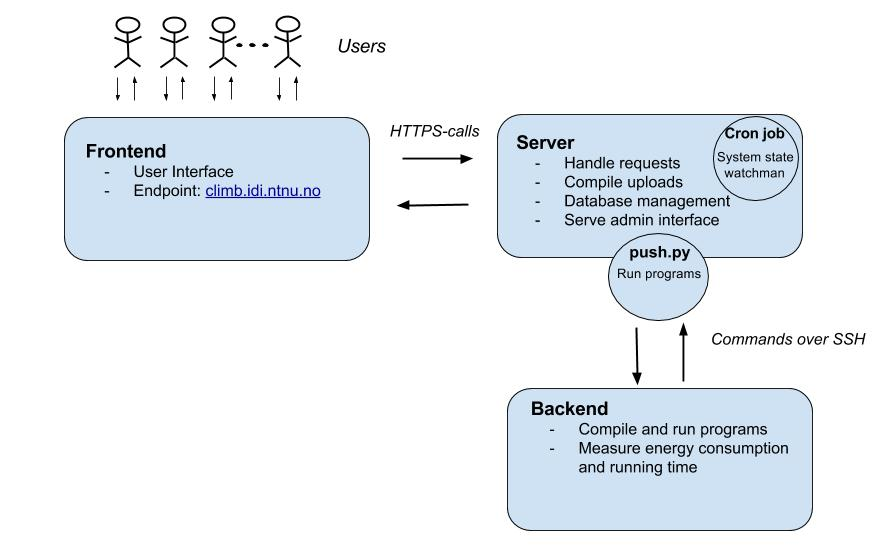
\includegraphics[width=1.0\textwidth]{figs/cmb_arch.jpg}
  \caption[The Climbing Mont Blanc system architecture.]{The Climbing Mont Blanc system architecture.}
  \label{fig:cmb_arch}
\end{figure}

\subsection{Frontend}
\label{subsec:cmb-arch-frontend}
The frontend handles all user based interaction. It is developed in AngularJS \cite{ANGULARJS}, which is a framework developed by Google and is maintained by Google and individual developers. The current frontend uses Angular version 1.3 and Javascript ECMAScript 5th edition. Angular is based upon the \gls{mvc} pattern \cite{b:mvc} and extends HTML with dynamic views with two-way data binding for building single page applications. The result is a smoother user experience, as views updates dynamically with model changes without the need of manually refreshing the web page. The framework also lets the developer define own reusable components, which in most situations make the code base more structured. The view structure and styling are defined in HTML5 and CSS3 respectively. Google Analytics, an advanced monitoring service provided by Google, monitors user interaction at the frontend. Among the things monitored is the number of active users, number of new users and user behavior. \\

\begin{figure}
    \centering
    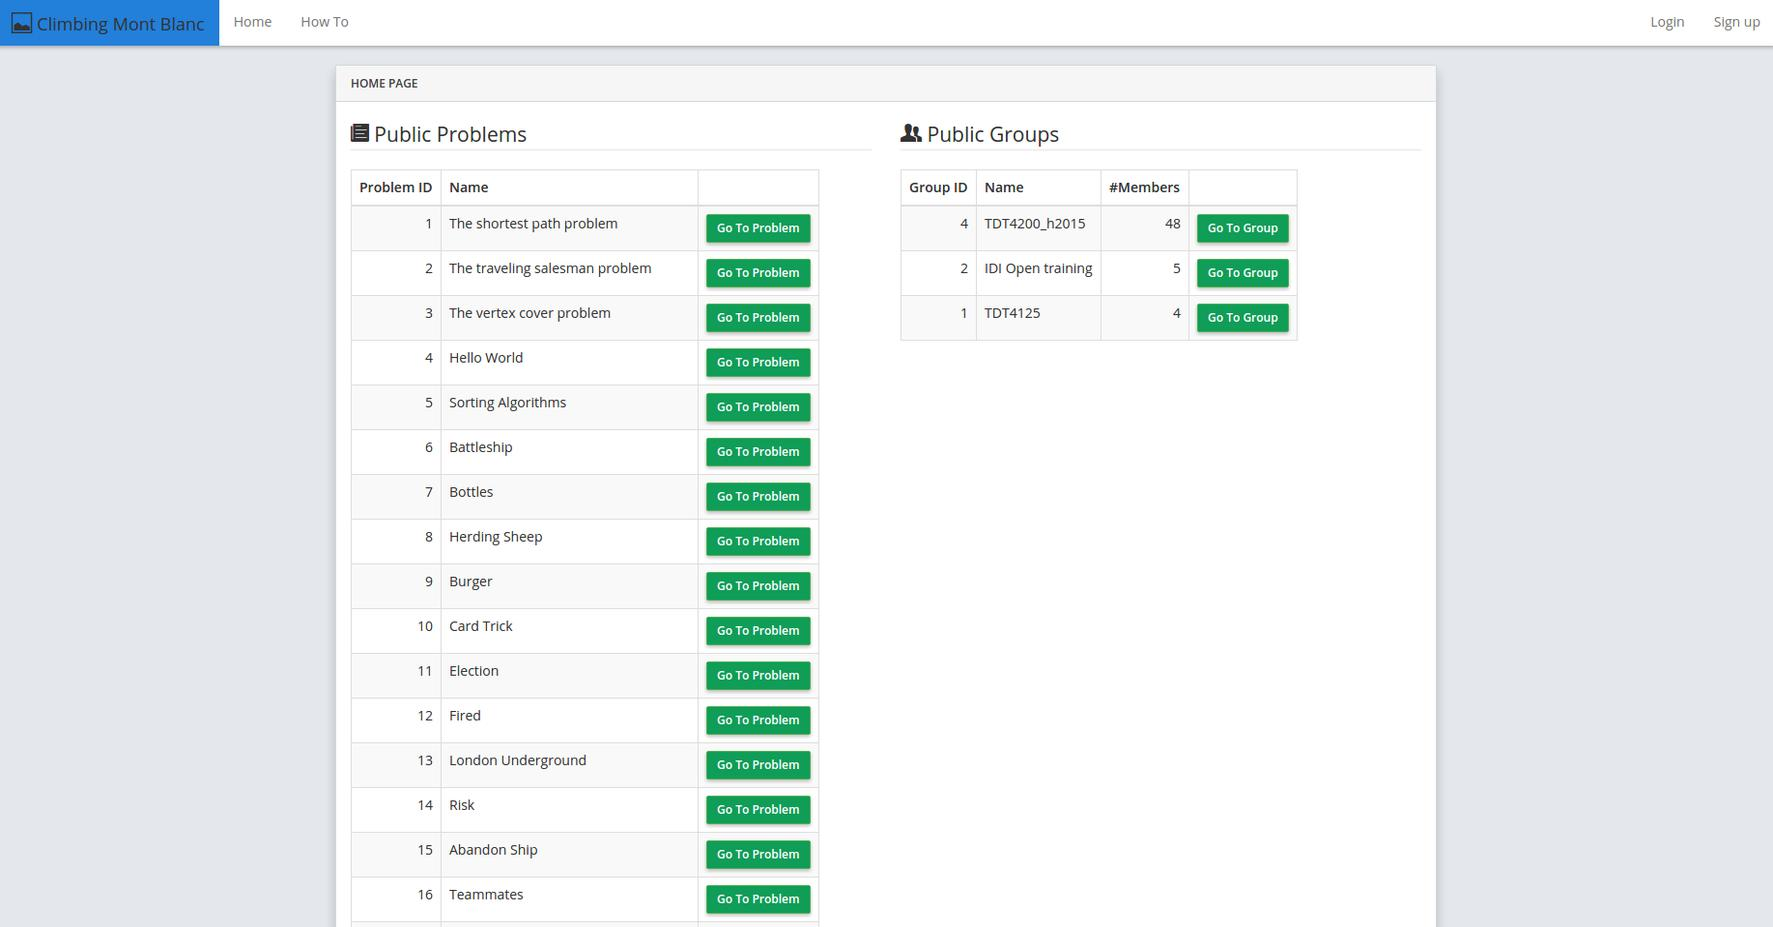
\includegraphics[width=1\textwidth]{figs/front_page.jpg}
    \caption{\gls{cmb} Home Page.}
    \label{fig:front-page}
\end{figure}

\begin{figure}
    \centering
    \begin{subfigure}[b]{0.82\textwidth}
        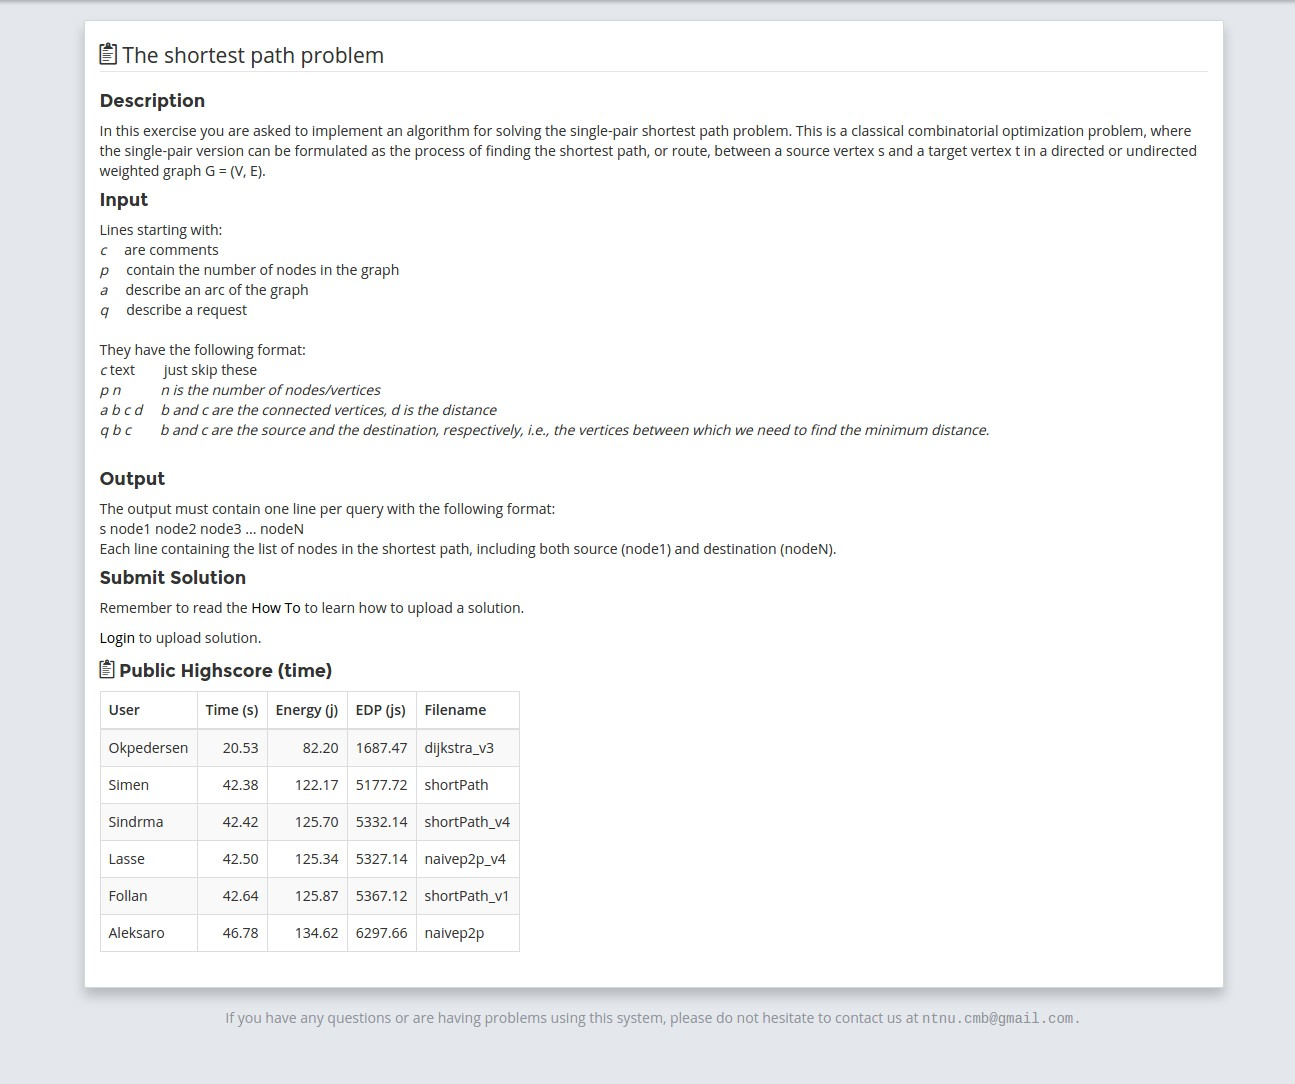
\includegraphics[width=\textwidth]{figs/problem.jpg}
        \caption{Problem View, logged out of \gls{cmb}.}
        \label{fig:problem}
    \end{subfigure}
    ~ %add desired spacing between images, e. g. ~, \quad, \qquad, \hfill etc.
    %(or a blank line to force the subfigure onto a new line)
    \begin{subfigure}[b]{0.82\textwidth}
        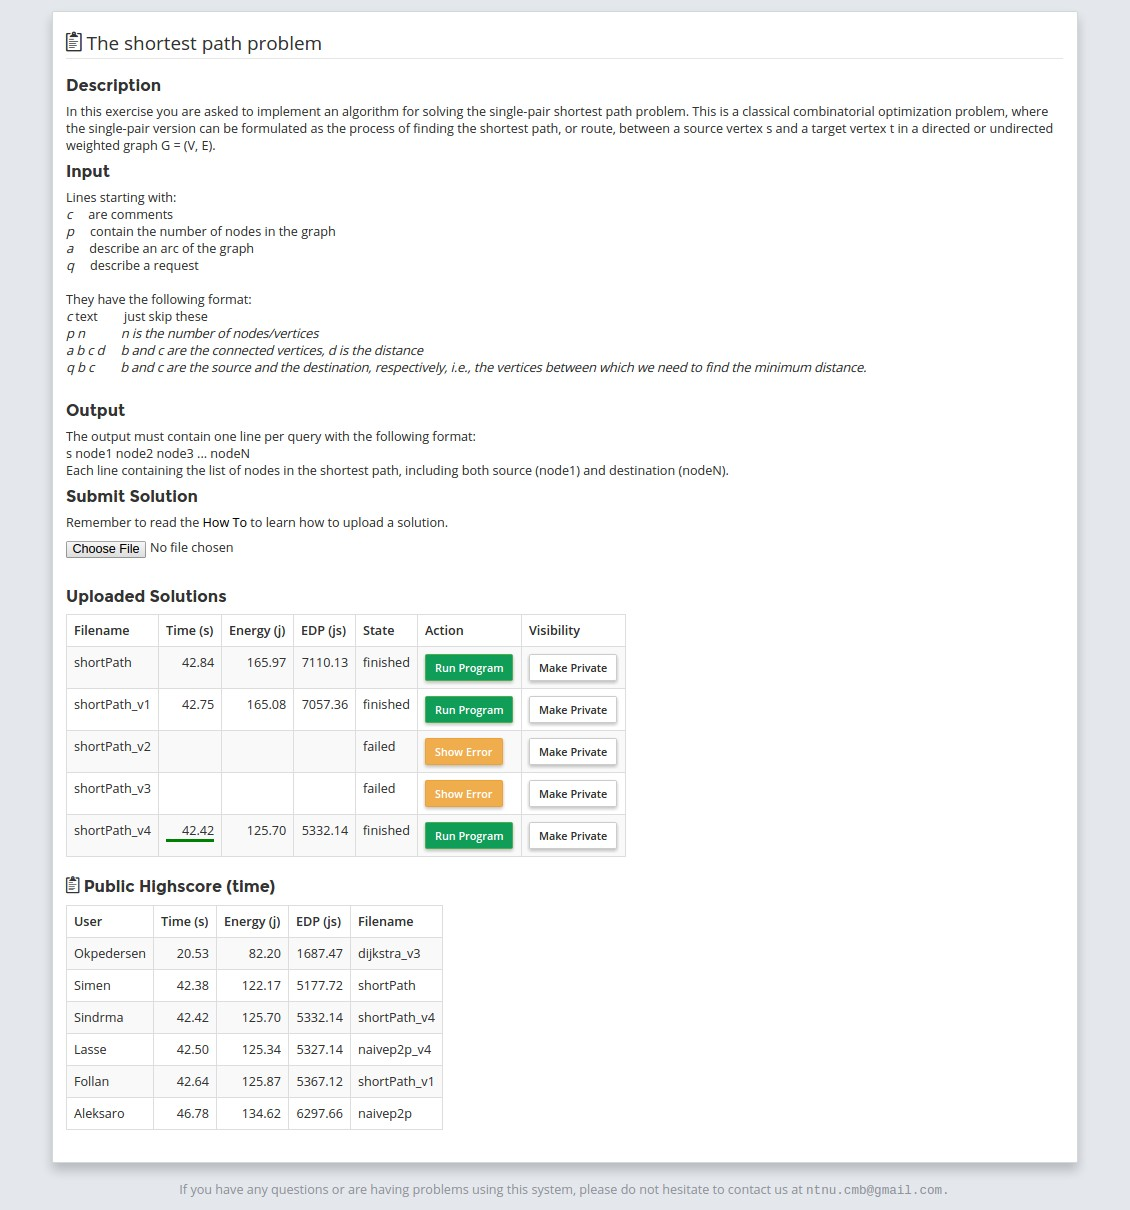
\includegraphics[width=\textwidth]{figs/problem_loggedin.jpg}
        \caption{Problem View, logged into \gls{cmb}.}
        \label{fig:problem-loggedin}
    \end{subfigure}
    \caption{\gls{cmb} Problem View States.}\label{fig:problem-view}
\end{figure}

The current system frontend can be reached at \url{https://climb.idi.ntnu.no} and the front page view is shown in Figure \ref{fig:front-page}. Appendix \ref{apdx:screenshots} shows screenshots of version one and two of the system frontend. Many actions against the frontend, such as routing to a different view, launches \gls{http} requests to the server that changes models and updates the views dynamically. Angular controllers make these requests to fetch up-to-date data to the frontend models or to update the database with changes made to the models by the user. Routing to a particular problem is an example of dynamic updates of the view, and also displays different views depending on the users state. If the user is not logged in, as shown in Figure \ref{fig:problem}, the view only shows the submitted programs that are \textit{visible}\footnote{A user may change the visibility of their submissions and results through the user interface.}. If the user then logs into the system, as shown in \ref{fig:problem-loggedin}, the problem view changes to make it possible to upload files and view previous submissions. Besides, many actions can be performed in the frontend like routing to a specific problem, login, sign up, create and join groups, manage groups, view the HowTo-page, see public problems and route to a particular problem to solve. The most common action is to upload possible solutions to a problem, which requires a zipped folder containing all source files. \\

\subsection{Server}
\label{subsec:cmb-arch-server}
The server is implemented as an \gls{rest} \gls{api}, as defined in by Roy T. Fielding et.al \cite{a:rtf}. The server is stateless, that is, the user state is stored at the frontend. It is also uniform, meaning that requests sent uses the same data format independent of the technologies used at the server and frontend. The \gls{rest}ful \gls{api} is implemented using Python Flask \cite{FLASK} and the data format used is \gls{json} \cite{JSON}. Our development and production servers also make use of Gunicorn \cite{GUNICORN} to handle simultaneous requests from multiple users. Gunicorn forks off multiple workers upon server startup, each having a private instance of the Flask webserver, and routes incoming requests to the current available workers. If no workers are available, the requests is stalled until a worker becomes idle. \\

Nginx \cite{NGINX} is used as a \textit{reverse proxy} on our development and production server. A reverse proxy serves static files on the fly while requests for dynamic content\footnote{Dynamic content is data that changes during runtime, such as database content.} are forwarded to Gunicorn. SQLite \cite{SQLITE} is used as database with SQLAlchemy \cite{SQLALCHEMY} on top. SQLAlchemy functions as an \gls{orm}, that is, it associates Python classes with database tables and objects of those classes with rows in the tables. SQLAlchemy makes it easy for the programmer to interact with the database, since SQL-statements are abstracted into Python objects and procedures. The underlying database schema is shown in Figure \ref{fig:old-database-schema}.\\

\begin{figure}
  \centering
  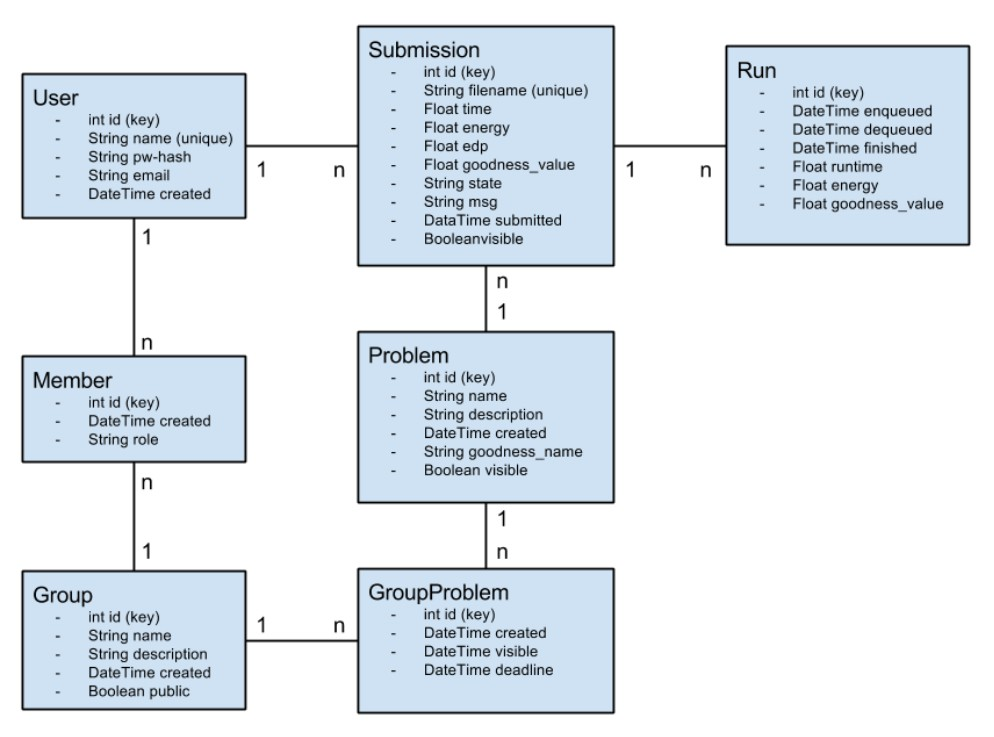
\includegraphics[width=1.0\textwidth]{figs/old_database_schema.jpg}
  \caption[Database schema.]{Database schema (taken from Master Thesis of Follan and Støa \cite{mt:T&S}).}
  \label{fig:old-database-schema}
\end{figure}

The server runs within a Python \textit{Virtual Environment} \cite{VIRTUALENV} that have all Python required dependencies\footnote{Dependencies is meant by dependencies in between packages (read: code libraries or code \gls{api}s). As an example, SQLAlchemy might require a specific version of Python Flask installed in order to work correctly.} installed. The virtual environment contains only the packages needed by the server, which removes potential dependency errors if the server is to host other Python-based systems in the future. The server is responsible for handling requests from the client, storing useful information in the database and filesystem, and compiling submitted programs. \\

A Python program called \texttt{push.py} runs in the background, regularly checking a \gls{fifo} queue for runnable programs. If a program is ready to run, the script will push the program from the server queue to the backend, and then compile and run it using \gls{ssh}. The result is returned to the server when execution terminates, and the server checks the correctness of the program before reporting the result back to the frontend. Further, the server is responsible for monitoring the state of the system with a background cron job. The cron job runs every 15 minutes, checking if the three system parts Gunicorn, \texttt{push.py} and backend is up and running. The system sends out an automatic e-mail to the system administrators in case of system failure. \\

The server also provides an administrator interface. Admin users have special privileges which grant them access to the admin interface found at \url{http://climb.idi.ntnu.no/admin}. Procedures that modify the database or the server file system are all done through the admin interface. The admins control a lot of the content visible on the frontend, such as programming problems visibility. The most common administrator operation is to add new problems, which requires the admin to add a new problem to the database and upload all files needed to the server. \\

The files needed to make a problem solvable are a input file to be piped into the submitted programs, a file that hold the expected result of an execution and a special file called \texttt{checker.cpp} that checks the correctness of submitted programs. When a program is executed, the input files are given as arguments to the submitted program. When the program is done executing, the checker compares the output of the submitted program against the expected answer files. The program is accepted if the checker program approves the program output. Since the checker is a regular C++-program, it is up to the admin to define what sort of output that should be accepted by the checker. Most of the problems available simply check the difference between output and expected output using the Unix \texttt{diff} program \cite{DIFF}. A special database field called \textit{goodness} can also be added to the problem. The database field is meant for approximation problems to check how ``good'' a solution is. As an example, a solution to the Vertex Cover problem might yield a different cover on each run. The admin making the problem can then define in the checker how good a given cover size is. More information on how to add problems through the admin interface can be found in Appendix \ref{apdx:problems}. 

\begin{sidewaysfigure}
    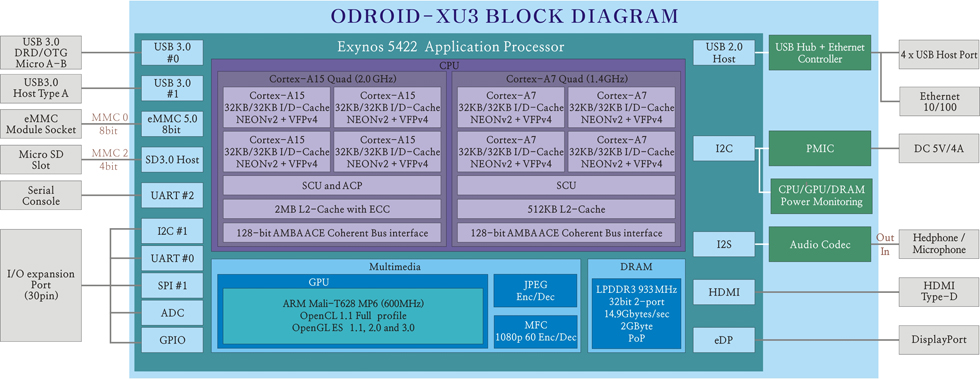
\includegraphics[width=1.0\textwidth]{figs/block-xu3.jpg}
    \caption[Odroid XU3 Block Diagram.]{Odroid XU3 Block Diagram (source: Hardkernel Website \cite{XU3-BLOCK}).}
    \label{fig:odroid-block}
\end{sidewaysfigure}

\subsection{Backend}
\label{subsec:cmb-arch-backend}
The backend is the executing unit of the CMB system. It is an Odroid XU3 board \cite{XU3} which consists of an Exynos 5 Octa heterogeneous multicore. A block diagram of the board is shown in figure \ref{fig:odroid-block}.  The Odroid board uses a minimal of the external interfaces and components available to get more consistent energy readings; the Ethernet port for internet access, eMMC module or MicroSD card for the \gls{os} image\footnote{The eMMC module loads the \gls{os} image faster than a MicroSD card, and is prefered over a MicroSD card if the module is functional.} and file system, and the board energy monitors. The Exynos 5 Octa consists of four big ARM Cortex A-15 and four small ARM Cortex A-7 cores which share the same \gls{isa}, but have different characteristics when it comes to performance and power consumption. The Exynos chip also has an ARM Mali-T628 GPU with six cores and combined with the two ARM processor types, which makes the Exynos chip a \textit{three-way heterogenous multicore with 14 cores}. \\

The Exynos chip makes use of ARM big.LITTLE technology. The technology enables the \gls{os} to perform Global-Task-Scheduling; to dynamically assign threads to the most appropriate CPU based on the run-time information \cite{ABL}. The board will compile and run the programs pushed to it by the server script \textit{push.py}, measuring time and energy as the program executes. Upon program termination, the board will calculate the program energy consumption and report results back to the server for further processing. The observant reader might view a compilation both at the server and at the board as redundant. Server compilation is done as the server has the capacity to handle multiple users simultaneously, and provides quicker feedback to the user in case of compilation errors. Also, the system lacks a good cross-compiler, and we have not found an appropriate cross-compiler for the server. The backend also needs to compile the submitted program, as the server and backend have different \gls{isa}s. The current CMB backend supports the programming languages C and C++, compiled with gcc-4.9 and g++-4.9 respectively. The compilers have support for both OpenCL v1.1, OpenMP 4.0, NEON and PThreads NTPL 2.19.


\subsection{Energy Measurements}
\label{sec:em-cmb}
The Hardkernel EnergyMonitor program is used to monitor power consumption and is compatible with Odroid XU3 \cite{OEM}. The pipeline in Figure \ref{fig:execution-pipeline} shows the execution pipeline when a program is pushed to the backend. The program is first compiled, and further executed on a small input set to detect potential runtime errors. If there are no runtime errors, the EnergyMonitor program is started and the cache is cleared. Due to energy consumption irregularities found by Follan and Støa \cite{mt:T&S}, clearing the cache is necessary to obtain stable energy readings. After the cache is cleared, the CPU is heated using the UNIX \texttt{stress} \cite{STRESS} command. The CPU runs \texttt{stress} to obtain a fixed start temperature (currently 60 degrees Celsius) before running the program. Starting benchmarks at the same temperature before each run of a benchmark is important to obtain stable energy readings, as pointed out by Cebrian and Natvig \cite{a:JL:T}. The current backend uses the sensors monitoring the temperature of the four big ARM Cortex A15 cores to arrive at the given target temperature of 60 degrees. The program is then executed and, upon program termination, the EnergyMonitor program is ended. Finally, after post processing the program power consumption, the result is reported back to the server. \\

\begin{figure}
  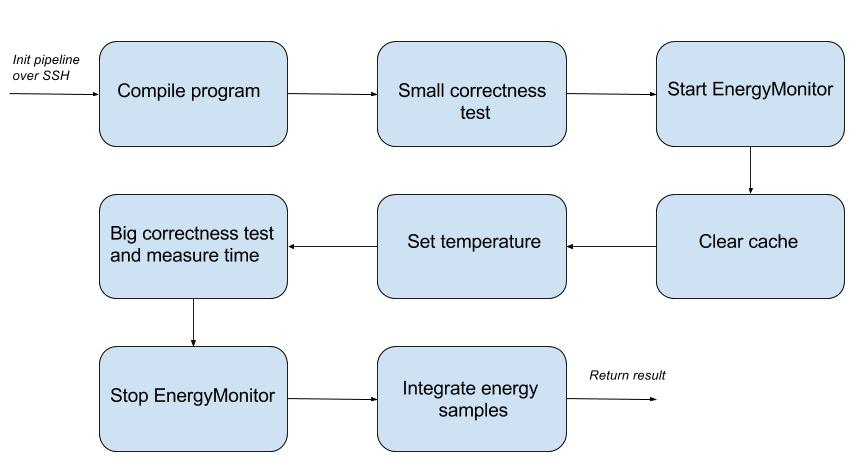
\includegraphics[width=1.0\textwidth]{figs/execution_pipeline.jpg}
  \caption[Backend execution pipeline.]{Backend execution pipeline (adapted from \cite{mt:T&S}).}
  \label{fig:execution-pipeline}
\end{figure}

Timestamps are captured right before and right after a program executes to measure execution time. The same timestamps are also used to fetch the power consumption during program execution, by parsing the output of the EnergyMonitor program and select the measurements captured for the big correctness test in the Figure. Upon receiving the results from the backend, the server then calculates the \gls{edp} \cite{a:edp}. This metric is chosen as it emphasizes both energy and performance. Energy is in itself a poor energy efficiency metric since we could simply run a program on a slow and under clocked CPU to obtain low energy consumption. \gls{edp} is defined in Equation \ref{eq:edp}, where \textit{E} is the energy used, \textit{D} is the delay or execution time.

\begin{equation}
  \label{eq:edp}
  EDP = E * D
\end{equation}

The observant reader might have noticed that the Mont Blanc project uses the metric FLOPS/W. This metric may be a useful metric when running the same benchmark, or implementation over and over again to test the energy efficiency of \gls{hpc} and processors architectures. However, \gls{cmb} compares different implementations on the same problems repeatedly, i.e the number of operations may differ from one implementation to the next. Another problem is to determine the number of \textit{useful} instructions, or in other words, instructions that contribute towards solving the problem. For these reasons, \gls{edp} is preferred over FLOPS/W in the \gls{cmb} system and is also the primary energy efficiency metric used in the system.

\begin{table}[b!]
  \centering
  \begin{tabular}{ l|p{2.1cm}|p{2.2cm}|l|l }
    & \textbf{Package Manager} & \raggedright\textbf{Test Framework} & \textbf{Linter} & \textbf{Other} \\ \hline
  \multirow{2}{*}{\textbf{Frontend}} & npm \cite{NPM} & Jasmine \cite{JASMINE} & jshint \cite{JSHINT} & gulp \cite{GULP} \\
                                     & bower \cite{BOWER} & Karma \cite{KARMA} &  &  \\ \hline
  \multirow{1}{*}{\textbf{Server}} & pip \cite{PIP} & nose \cite{NOSE} & flake8 \cite{FLAKE8} & virtualenv \cite{VIRTUALENV}\\
  \end{tabular}
  \caption{\gls{cmb} code correctness tools.}
  \label{tab:cct}
\end{table}

\subsection{Code Correctness and Code Deployment}
\label{sec:cmb-ci}
Unit test frameworks and other tools are used to ensure code correctness in both the frontend and server code. The tools used by the \gls{cmb} system is summarized in table \ref{tab:cct}, and are split into four categories. \textit{Package Managers} are used to install and upgrade dependent code packages and libraries used by the system. The required code packages needed are all listed in special files, one unique file per package manager. Both the frontend and server code makes use of \textit{test frameworks} to develop and run unit- and integration tests and there exist multiple unit tests on both system components. \textit{Linters} are special tools that ensure that language standards are followed, such as semicolons at the end of each line in Javascript or correct indentation in Python files. Other tools include gulp \cite{GULP}, which is a small build system used at the frontend that can execute small user defined tasks, such as running the frontend linter and unit tests or compressing the HTML, CSS, and Javascript files. At the server, virtualenv \cite{VIRTUALENV} is used as a virtual environment as described in Sub-\Cref{subsec:cmb-arch-server}. \\

To quickly deploy new features, the system makes use of \textit{Jenkins} \cite{JENKINS} as \gls{ci} server or build server. \gls{ci} is a software engineering practice that automates the testing and deployment of systems. Fowler reports some benefits of CI in his article from 2006; a clone of the production environment (so-called development server) runs tests on the code changes before deployment to production, bugs are discovered and removed easily, and as a whole it makes it possible with rapid integration of new features \cite{a:F:CI}. As briefly mentioned in Sub-\Cref{subsec:cmb-arch-server}, the \gls{cmb} system has a development and production server, and these are used to implement \gls{ci} as a practice in the project. The development server is used for manually testing new features in a production-like environment as features are developed. Features that passes the manual testing stage are then deployed to the \gls{cmb} production server. Jenkins can be configured to fit into various system environments, and Figure \ref{fig:server-ci} summarizes its use-case in the \gls{cmb} system. \\

\begin{figure}
  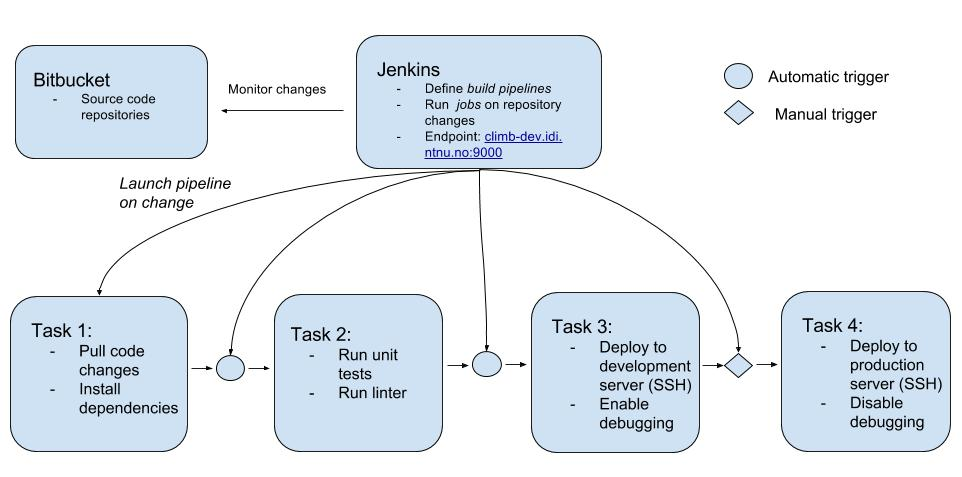
\includegraphics[width=1.0\textwidth]{figs/build_pipeline.jpg}
  \caption[Build pipeline.]{Build pipeline.}
  \label{fig:server-ci}
\end{figure}

The Jenkins \textit{build pipeline} in Figure \ref{fig:server-ci} is defined for both the frontend and server code. Each step in the pipeline is called a \textit{task}, and may have various configurations and use-cases depending on the system environment. The tasks shown in the Figure demonstrates the task configurations used in the \gls{cmb} system. The first task in the pipeline is launched upon code changes on the master-branch in the respective git-repository. The task pulls all the new code changes from git and ensures that installation of package dependencies does not crash the system. If the first task completes without errors, it will automatically trigger the next task which will run all defined unit tests and the linter. As before, if there are no errors, task three is launched which deploys the recent changes to the development server over \gls{ssh} with debugging enabled. If the third task is successful, the code changes should be visible on the development server of \gls{cmb}. \\

Manual acceptance testing and integration tests can be carried out. If the developer(s) are satisfied with the new features, the final and fourth task can be triggered manually. The task deploys the changes to the production server of \gls{cmb}, which also takes care of disabling debugging and compressing the frontend code. Disabling debugging and doing frontend code compression minimizes the number of requests made by the browser and makes the server code execute faster, and it is important to note that this does not affect the functionality of the system. The development server does, as mentioned, have debugging enabled, and uncompressed code to easier find bugs during acceptance testing. Since the difference between the two servers does not sacrifice the functionality of the system, it does not violate the rules set by \gls{ci}.  \\

The \gls{cmb} development server has the a Jenkins server installed and provides a user interface available at \url{http://climb-dev.idi.ntnu.no:9000}.All development should be done locally and then merged with the code on Bitbucket to follow the practice of \gls{ci} correctly. It is considered bad practice to develop code on the development or production server, and the reader should refer to Appendix \ref{apdx:setup} to learn about system setup and local development.

\subsection{Security}

\paragraph*{User Information Security} A number of security measures are taken to make sure that user data are stored and accessed safely. The password is processed by the Python Werkzeug security package \cite{WERKZEUG} upon user creation, to ensure that the password is salted and hashed before being stored in the database. This procedure executes upon both regular and admin user creation. Equal passwords will generate the same hash, but it is very hard for adversaries to reconstruct a password hash. The user sends the password in the login request made to the server \gls{api}, and becomes authenticated if the password hash matches the hash stored in the database. The server then returns a \textit{token}\footnote{A token is some unique string valid for a specific period of time.} which contains enough information to describe uniquely a user-session, and it is sent back in a HTTP response header named \textit{Authorization}. The token is required in some of the requests made to the server \gls{api}, such as uploading and running submissions, and the frontend code takes care of including the header before such requests are made. The token is valid for one hour, which requires a new login after an hour of inactivity. \\

Since the token is stored at the frontend, the server is \textit{stateless} and thereby \gls{rest}ful as mentioned in Sub-\Cref{subsec:cmb-arch-server}. To make the transfer of information even more secure, \gls{https} is used to encrypt all the information sent in requests between the server and frontend. \gls{https} use \gls{ssl} to encrypt messages sent to and from the server and is almost impossible to decrypt, which enables safe transfer of passwords and other sensitive data between the server and frontend.

\paragraph*{Uploaded Programs Security} Uploaded program can potentially contain malicious code either in the source files or file names. To restrict the number of possible actions that can be made through the uploaded code, the backend executes the code using a Unix user named \textit{worker} that has minimal \gls{os} permissions on the backend. Also, to remove possible malicious scripts residing in file names, the server again makes use of the Python Werkzeug security package \cite{WERKZEUG} before storing the files in the server file system. It might be worth mentioning that it might be an idea to further extend the system with designated compile servers or threads since unknown errors during compilation might crash the server. Since no such error has occurred, it is listed in Appendix \ref{apdx:backlog} as a possible feature to be added to the system at a later point.

\paragraph*{System Security} The reverse proxy server used at the server is configured to handle \gls{https} requests. As mentioned, the server uses \gls{ssl} when sending and receiving \gls{https} requests. SSL requires an SSL Certificate to work, which is a guarantee that the holder of the certificate provides trustworthy and safe web-content. The most common browsers have a list of trusted third parties issuing certificates, called \glspl{ca}, and every certificate issued by one of the \glspl{ca} on the list are trusted as safe. Uninett is one example of a \gls{ca} and has created the SSL certificate that is used by the \gls{cmb} system. Since Uninett is a well known \gls{ca}, the \gls{https} requests sent by the system is trusted by most browsers. \\

The \gls{cmb} backend also has \gls{ufw} \cite{UFW} installed. \gls{ufw} which restricts access to the board by requiring every \gls{ssh} request to originate from within the NTNU network. The backend also has Fail2ban  \cite{FAIL2BAN} installed, which restricts the number of authentication attempts made within a certain timeframe. If there are more than three attempts from the same IP-address within the configured timeframe, the IP-address is banned from sending requests for 10 minutes. The server also has \gls{ufw} and Fail2ban installed, but the setup of \gls{ufw} is slightly different. The server \gls{ufw} setup allows all requests made to port 80 and 443 to enable the requests made to \gls{http} and \gls{https} respectively. The setup makes the CMB frontend is accessible from outside the NTNU network. To keep up to date with security updates \texttt{unattended-updates} \cite{UNATTENDED} is enabled on the production server, which installs security updates if needed. The check for security updates are made every night at 02:00, and an automatic restart of the system is done if the update requires it.


\subsection{Other Related CMB Projects}
\label{subsec:related-proj}
\begin{figure}[ct!]
  \centering
  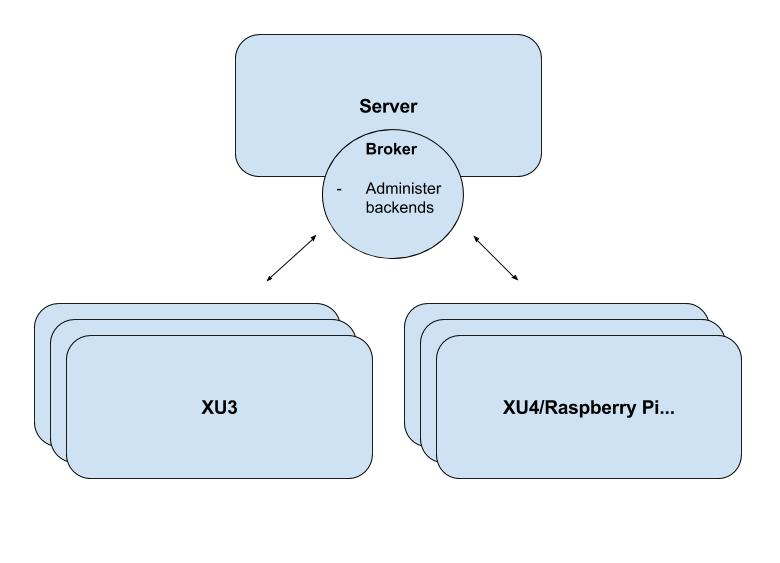
\includegraphics[width=0.7\textwidth]{figs/cmb_scale_arch.jpg}
  \caption[Scalable \gls{cmb} architecture.]{Scalable \gls{cmb} architecture.}
  \label{fig:cmb-scale-arch}
\end{figure}

\subsubsection{System Scalability}
Previous user testing has shown that the system is bottlenecked by the number of executing units. The bottleneck was noticed during the Autumn of 2015 when students had to use the system as part of mandatory exercises in the course TDT4200 Parallel Computing \cite{TDT4200}. The Specialization project report delivered in December 2015 presented feedback given by the TDT4200 students, and some students pointed out that submissions often stalled for several minutes in the run queue with little feedback on progress. Even though students were advised to start exercises early and submit to the system long before exercises were due, the system should still handle a higher load of users duringthe last few hours before the exercises' deadline. Further, if the system is to be used in programming competitions like \gls{icpc} \cite{ICPC} or IDIOpen \cite{IDIOPEN} as well, it needs to handle multiple concurrent submissions without stalling them in the queue for to long. \\

The observations motivated the extension with several execution backends like depicted in Figure \ref{fig:cmb-scale-arch}. Christian Chavez has been assigned the thesis on \gls{cmb} scalability, which should extend the system with more Odroid XU3 boards. The idea is to have multiple backends at the \gls{cmb} production server to handle multiple submissions at the same time, as described in the CMB paper by Natvig et.al \cite{a:CMB}. A control mechanism needs to be implemented, to administer the incoming requests and possible run queue race conditions. This mechanism is called a \textit{broker} in Figure \ref{fig:cmb-scale-arch}. Have in mind that the figure describes the concept of scaling the system with multiple boards, and there are several possible ways to implement the suggested broker. \\

Follan and Støa suggested that one could simply add more push scripts, one script for each connected backend \cite{mt:T&S}. While this solves the problem of extending the system with more boards, the push script has proven to fail and terminate due to some erroneous output from the backend. Finding errors and bugs in bash scripts executed over \gls{ssh} in Python has proven to be difficult to debug, which has driven the project team to look for other solutions than simply extending with more push scripts. The Specialization project report proposed the use of \textit{task queues}, which are mechanisms to distribute work among threads or machines. However, it might impose unnecessary complexity to the system.  \\

The thesis will also describe how the broker can be used to allow different backends other than the currently used Odroid XU3 board. Figure \ref{fig:cmb-scale-arch} also shows an illustration of the architecture if extended with different backends. Allowing various types of boards on the system enables further exciting research on energy efficient programming, and may provide \gls{cmb} users with the possibility of comparing the energy efficiency of benchmarks on multiple architectures in a quick manner.

\section{Related Work}
\label{sec:related}
This section will present related \glspl{oj} which might inspire the future development of the \gls{cmb} system. The presented work is inspired by the \glspl{oj} presented in the master thesis of Follan and Støa and further extended with interesting \glspl{oj} as well as the \glspl{oj} mentioned in the Specialization project. There exists many \glspl{oj} sites which have a wast amount of users and submissions, but as mentioned, we are not aware of any other \gls{oj} focusing on energy efficient programming. Instead, we present popular \glspl{oj} and their features, which might have an effect on the future development of \gls{cmb}. Further, we also present the most popular crowdsourcing sites as these have some relevance to the project. Table \ref{tab:definitions} lists the definitions of an \gls{oj} (briefly mentioned in \Cref{sec:cmb}) and crowdsourcing. Since crowdsourcing is a broad term we will further restrict the definition: \textit{Crowdsourcing is the action of outsourcing programming tasks and problems to a large group of programmers in the form of an open call}. The definitions are valid throughout the thesis. \\

%The most relevant work we have found within energy efficient programming is the Green Coding contest \cite{GREENCODING} hosted in 2014. However, we have not been successful in finding results from this competition and it has only been hosted once. Instead, we present some of the most relevant work within Energy-Aware programming and software in sub \Cref{subsec:eap}, focusing on work which might effect the energy efficiency measurements and software we have developed to the Odroid XU3.
\begin{table}[t!]
    \centering
    \begin{tabular}{ | l | p{7cm} | }
    \hline
    \multicolumn{2}{ | c | }{\textbf{Definitions}} \\
    \hline
    Online Judge & ``An online based computer system, providing programming problem descriptions and data sets to automatically judge wether a particular solution solves a given problem.'' Inspired by definition found in \cite{a:Kurnia2001}  \\ \hline
    Crowdsourcing & ``The act of taking a job traditionally performed by a designated agent and outsourcing it to an undefined, generally large group of people in the form of an open call.'' \cite{CROWDSOURCING}. \\ \hline
    \end{tabular}
    \caption{Defining \glspl{oj} and Crowdsourcing}
    \label{tab:definitions}
\end{table}
%\subsection{Online Judges and Crowdsourcing}
%\label{subsec:oj&c}
%Torbjørn Follan and Simen Støa mentioned several of the most popular \glspl{oj} in their Master Thesis \cite{mt:T&S}. The In-Depth study delivered in December 2015 summarized the \glspl{oj} mentioned by Follan and Støa, and further explored trending \glspl{oj} not previously presented. This sub-section will present the \glspl{oj} both presented by Follan and Støa and in the In-Depth study, focusing on unique features and aspects that may inspire the future development of the \gls{cmb} \gls{oj}. The In-Depth study also mentioned the most popular Crowdsourcing websites, and the crowdsourcing sites mentioned in that work will also be briefly introduced in this sub-section. Table \ref{tab:definitions} presents the definitions of an \gls{oj} (mentioned in \Cref{sec:cmb}) and Crowdsourcing, which are valid throughout the thesis. The definition of crowdsourcing is broad, and in this thesis it is further restricted: Crowdsourcing is the action of outsourcing programming tasks and problems to a large group of programmers in the form of an open call. As mentioned earlier, we are not aware of any other \glspl{oj} which focuses on energy efficient programming. The Green Coding contest \cite{GREENCODING} hosted in 2014 is the only work we have found related to energy efficient programming. This sub-section summarizes the \glspl{oj} that is either very popular or has unique factors compared to other \glspl{oj}, and in addition present the most popular crowdsourcing sites within information technology relevant for the CMB project.
\paragraph*{Kattis} \hfill \\
The first version of Kattis was developed in 2005 at KTH in Stockholm \cite{a:Enstrom2011}. The judge was first used for assessing programming exercises in various courses at the university. Since the first version, the Judge has developed into a sophisticated and well known \gls{oj} and is widely used in the Nordic countries, perhaps because of its usage in the programming contests \gls{icpc} \cite{ICPC} and IDIOpen \cite{IDIOPEN}. The judge supports 13 programming languages and offers a broad range of programming problems to solve with varying difficulty. The judge is offered to the public through a website, but it is also offered as a simple \gls{cli}.\footnote{The Kattis \gls{cli} can be found at github: \url{https://github.com/Kattis/kattis-cli}.} \\

Kattis also offers services for firms and universities alongside hosting an public \gls{oj}. Professors can register courses and automatically grade programming exercises, such that students easily can get feedback and track their exercise scores. The service also offers plagiarism checks of submitted code and analytics of the registered courses. Companies can register to challenge potential job candidates with a set of programming problems before interviewing them, and offer crosschecking of submitted code to filter out cheaters. The universities can choose either a free subscription with a limited number of registered courses and teachers, or a premium subscription with an unlimited number of teachers and courses with a cost of 15\$ per student, per course. Companies have three different paid subscriptions to choose from, which offers either a few, medium or large number of interviewers and problems depending on the chosen subscription.

\paragraph*{UVa Online Judge} \hfill \\
The first version of UVa Online Judge \cite{UVA} was developed by former student Ciriaco García de Celis in 1995 \cite{a:Revilla2008}. The judge was first built as a series of bash scripts, but the scripts were later replaced by a team of students to make the judge able to handle the increasing amount of submissions and to ready the system to be used in programming competitions. Today the UVa Online Judge is very popular, with over 1,8 million submissions registered in 2015 and over 100,000 users. The judge also offers over 4,300 programming problems solvable in 6 different programming languages.

\paragraph*{PKU JudgeOnline} \hfill \\
PKU JudgeOnline \cite{PKU} released in 2003 and is one of the \glspl{oj} with the highest number of submissions. At its peak in 2010, the judge had over 1.768 million submissions, but the number of submissions has decreased in recent years measuring almost 1,3 submissions in 2015. The \gls{oj} provides mostly the same features as other \glspl{oj}, like viewing statistics, submitting code to problems, and hosting online contests.

\paragraph*{URI Online Judge} \hfill \\
The URI Online Judge is served through a website which was first presented in July 2012 \cite{a:Bez2013}. The \gls{oj} aims to support both teaching student about programming and professors aiding them to manage courses and exercises. A total of eight problem categories is offered, training students in various topics in programming. Bez et.al also mentions a couple of features implemented. One feature lets the user send in the input test cases to a problem, in which the online judge responds with the correct expected output. Another lets the user view the code directly in the browser during compilation errors, with highlighted code lines on those lines containing errors \cite{a:Bez2013}.

\paragraph*{HackerRank} \hfill \\
HackerRank \cite{HACKERRANK} has over 800,000 developers registered and over 800 public problems and challenges. The project was started in 2008 by Vivek Ravisankar and Hari Karunanidhi. The founders felt like they spent too much time on engineering interviews and less time creating great solutions, and they also had a hard time finding good programmers through the traditional interview process. The \gls{oj} supports over 35 programming languages and offers a clean design in their interface, with features such as online code editing. HackerRank does also have an extensive work section with more than 1,000 companies registered. The companies interested in filling a particular position can create a basic free profile to interview candidates, create or add problems, and watch the candidate code in real-time. One can also request a premium subscription, which has even more advanced features like detecting code plagiarism. It does also have a section for schools that want to create online programming assignments similar other judges providing the same feature.

\paragraph*{HackerEarth} \hfill \\
HackerEarth \cite{HACKEREARTH} has over 14.4 million submissions, 3,146 practice problems, and 232 in-depth tutorials. The HackerEarth team has one goal: make technical recruitment straightforward and efficient. The judge offers much of the same features as HackerRank and the other \glspl{oj} mentioned above but has some unique features as well. They provide a \gls{rest}ful \gls{api} documentation, which can be used to integrate the \gls{oj} with other software systems. The HackerEarth team has also developed a chrome extension to notify their users about upcoming programming competitions and events. The judge also hosts programming competitions, provide practice problems, provide a similar extensive work section as HackerRank, and provide multiple technical and non-technical blogs. HackerEarth can also be seen as a partial crowdsourcing site, with its numerous challenges and hackathons provided by firms on the HackerEarth website.

\paragraph*{LeetCode} \hfill \\
LeetCode \cite{LEETCODE} has about 52,000 users registered. Their goal is to prepare coders for technical IT interviews, and offer much the same features as the other \glspl{oj} above. However, they have a unique feature which is in-depth articles per problem. Each article goes into depth about the theory required to solve the given problem, and the \gls{oj} also enables its users to discuss the articles with other users through their online forum.

\paragraph*{Other popular \glspl{oj}} \hfill \\
There are three more Online Judges that is worth mentioning briefly. These are Timus Online Judge \cite{TIMUS}, A2 Online Judge \cite{A2OJ}, CodeChef \cite{CODECHEF}, and Sphere online judge \cite{SPHERE}. These \glspl{oj} offer features similar to those already presented, so they are not explained in great detail. More information about them can be found on their websites.

\paragraph*{TopCoder} \hfill \\
The crowdsourcing site that seems to be the most popular is TopCoder \cite{TOPCODER}. The site got more than 895,000 members and is used by companies like Amazon, Facebook, IBM, and Microsoft for crowdsourcing real world problems to solve. The best solutions to a problem often get awarded with a money prize.

\paragraph*{RecSys Challenge} \hfill \\
The RecSys Challenge \cite{RECSYS} is a crowdsourcing competition that has been hosted every year since 2010. The competition aims to solve different challenges within recommender systems, where the top three winners receive a money prize and an opportunity to present their solution at the RecSys Conference. Many students at NTNU compete in this competition as a part of their master thesis.

%\subsection{Energy-Aware Programming and Software}
%\label{subsec:eap}

%Simon Holmbacka++ for accurate energy readings and
% fill in with more if discovered
% spørre Lasse om tips her, trenger flere kilder og helst artikler

%!TEX root=../main.tex
\chapter{Related Work}
\label{ch:related}

\section{Data Generation Method}

\section{Online Judges and Competitions}

% fill in with more if discovered
% spørre Lasse om tips her, trenger flere kilder og helst artikler

%!TEX root=../main.tex
\chapter{Climbing Mont Blanc Usability Goals}
This chapter starts with a definition of usable software systems in section \ref{sec:usability-def}. The section will define usability, and show a few aspects and characteristics in other \glspl{oj} which makes them usable with respect to the definition presented. Section \ref{sec:cmb-usability} ends the chapter with a discussion of usability goals for the \gls{cmb} system set by this thesis, aiming to further extend the \gls{cmb} system usability.

\section{Usability in Online Judge Systems}
\label{sec:usability-def}
Usability is defined in the ISO 9241 standard Part 11 as ``the extent to which a product can be used by specified users to achieve specified goals with effectiveness, efficiency, and satisfaction in a specified context of use.'' \cite{ISO1998}. The definition is broad and covers many aspects of a product, or in our case a software system. Usability is a broad term and can be hard to define precisely, however, literature seems to agree that the following five characteristics describe a usable software system  \cite{holzinger2005, ferre2001}; \textit{learnability}, \textit{efficiency}, \textit{user retention over time}, \textit{error rate}, and \textit{satisfaction}. A quick summary of each characteristic is summarized below.

\paragraph*{Learnability:} The users ability to learn to use the system. Learnability also involves the users ability to gain efficiency in using the system and reach their objectives in a quick manner.

\paragraph*{Efficiency:} Users should be allowed to obtain a high level of productivity when using the system. The usability is improved if the user can quickly reach their goals when using the system.

\paragraph*{User Retention Over Time:} The user should be able to return to the system after a break from using it, and remember the core functionality of the system. A usable software system makes it easy to get back into an efficient state without the need to learn the core functionality of the system anew. The characteristic is also refered to as \textit{memorability}.

\paragraph*{Error Rate:} The number of errors a user makes along the path of actions before reaching his or hers goal. A low error rate among users improves the usability of the system.

\paragraph*{Satisfaction:} The users subjective thoughts about the system as well as making the system pleasant to use. Satisfaction may involve functionality that is both visible and invisible through the system frontend. \\

Another related term to system usability is the notion of \textit{affordance} of things, which is defined by Donald Norman as ``the perceived and actual properties of the thing, primarily those fundamental properties that determine just how the thing could be used'' \cite{norman1988design}. Good affordances of entities and components in software systems will improve learnability, efficiency, memorability, and user satisfaction while lowering error rates, and thereby improve the usability of the system. \\

The definition of \glspl{oj} as presented in section \ref{sec:related} is quite straightforward. However, because of its simplicity, it is fairly important that the \gls{oj} is highly usable when users are actively using the system to solve programming problems. The most time-consuming tasks done by most users in an \gls{oj}, at least in the \gls{cmb} system, is to read problem descriptions as well as submit code for automatic judgement. The time spent on reading and submitting is minimalistic compared to the time spent on developing code, and code development often happen off site in an offline environment if not explicitly offered by the \gls{oj}\footnote{Some of the mentioned \glspl{oj} has web based code editors, such as Kattis \cite{KATTIS} or HackerEarth \cite{HACKEREARTH}}. \\

The action of uploading code is one of the main actions done by users. Making the action of uploading code simple is important for both efficiency and learnability. \glspl{oj} like HackerEarth makes it easy to upload code, providing an online code editor which can compile and test the code or directly submit a solution like shown in Figure \ref{fig:hackerearth-upload}. The user also has the option of uploading source files directly, which makes it easier for the users wanting to submit source files instead of coding directly in the browser. Presenting multiple alternatives in a structured way to users makes it simpler to use the system, as a given user may choose the method he or she is most comfortable with. The upload feature also shows good affordance, and the user knows by instinct how to submit code. \\

\begin{figure}
    \centering
    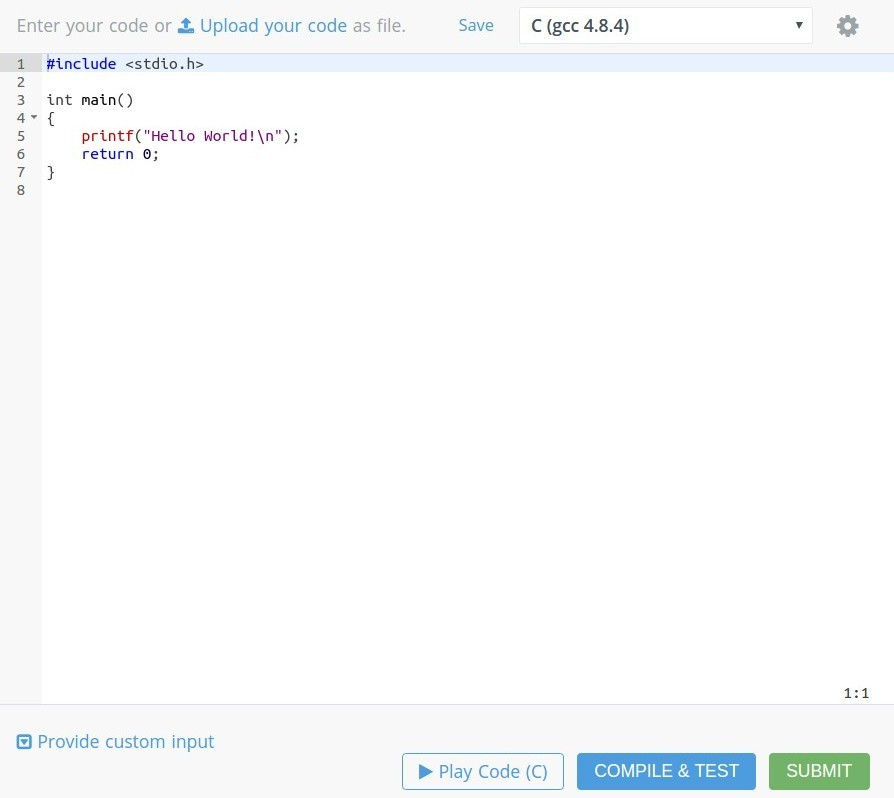
\includegraphics[width=0.8\textwidth]{figs/hackerearth_upload.jpg}
    \caption[HackerEarth Code Upload]{HackerEarth Code Upload (source: HackerEarth Website \cite{HACKEREARTH})}
    \label{fig:hackerearth-upload}
\end{figure}

It is also important that the user gets feedback on the state of submitted program. Tracking the state and repeatedly report to the user whenever the state of the submission changes is critical. It does not have to be very detailed, as long as the user get some notion of the state of the program. For example, Kattis does not automatically report the state of a submitted program, but they display a type of progress bar which is updated whenever test cases pass, and the user manually refreshes the current view. However, the more information displayed about critical data such as the state of the submission, the better. \\

The different components in the user interface should also respond as expected and give logical feedback. Failing to do so might distract the user, and thereby blocking the user from reaching his or hers goal. Norman mentions in his book that it is important that all actions made against the system should ``give an immidiate and obvious effect'' in the form of feedback to the users \cite{norman1988design}. For \glspl{oj}, this means clearly stating feedback and making the feedback visible for the users, as well as presenting useful and descriptive feedback messages.\\

Administrator users is also a part of the user group. Usability in \glspl{oj} also involves making the system usable for system administrators and problem makers, and it is important that admin interface usage is simple and understandable. Usage of a given admin interface likely require some training and knowledge about the system, but the interface should be simple, so users do not have to relearn how to use the system and quickly achieve high efficiency, i.e. high user retention over time. \\

Other features implemented by the judge should also behave as expected and the interface should be logically built. The \glspl{oj} presented in chapter offers various features and going into depth about the usability of this features is outside the scope of this thesis. However, it is worth mentioning that the \glspl{oj} should build the system with components with good affordances as described above. The professional \glspl{oj} mentioned in section \ref{sec:related} all have teams of developers and designers and offer simple and usable interfaces for their judges.

\section{Climbing Mont Blanc Usability Goals}
\label{sec:cmb-usability}
% Dra inn målene presentert i kapittel 1, og si motivasjonen til at det blir implementert med hensyn på seksjonen over.
Ease of use + performance + quick response + feedback

%!TEX root=../main.tex
\chapter{Climbing Mont Blanc Improvements}
\label{ch:improvements}

In this chapter it is assumed that a web interface follows the \gls{mvc} pattern. As briefly mentioned in sub-section \ref{subsec:cmb-arch-frontend}, Angular structures the HTML and Javascript code according to the \gls{mvc} pattern, and the reader should have the abstraction in mind when reading about browser or frontend implementations.

\section{Real Time Updates}
\label{sec:real-time}
The frontend view changes when a user performes actions against the frontend models as mentioned in sub-section \ref{subsec:cmb-arch-frontend}. However, the frontend view presented to a given user does not update automatically as other users interract and changes their data models, as models is stored locally in each of the user's browser. If the updated model contains data that should be known\footnote{Hereby known as \textit{shared data}.} to all users, the users does not get notified about the model changes dynamically and views may therefore display out of date information. Figure \ref{fig:update-problem} shows an example of the problem, as Alice updates some of her browser's model data when she interacts with the system. If Alice changes some data present in Bob's models, Bob will not be notified of the changes as all data transfer are done with HTTP requests between Alice and the server. However, Bob can fetch up to date data by manually refreshing his webpage. \\

\begin{sidewaysfigure}
    \centering
    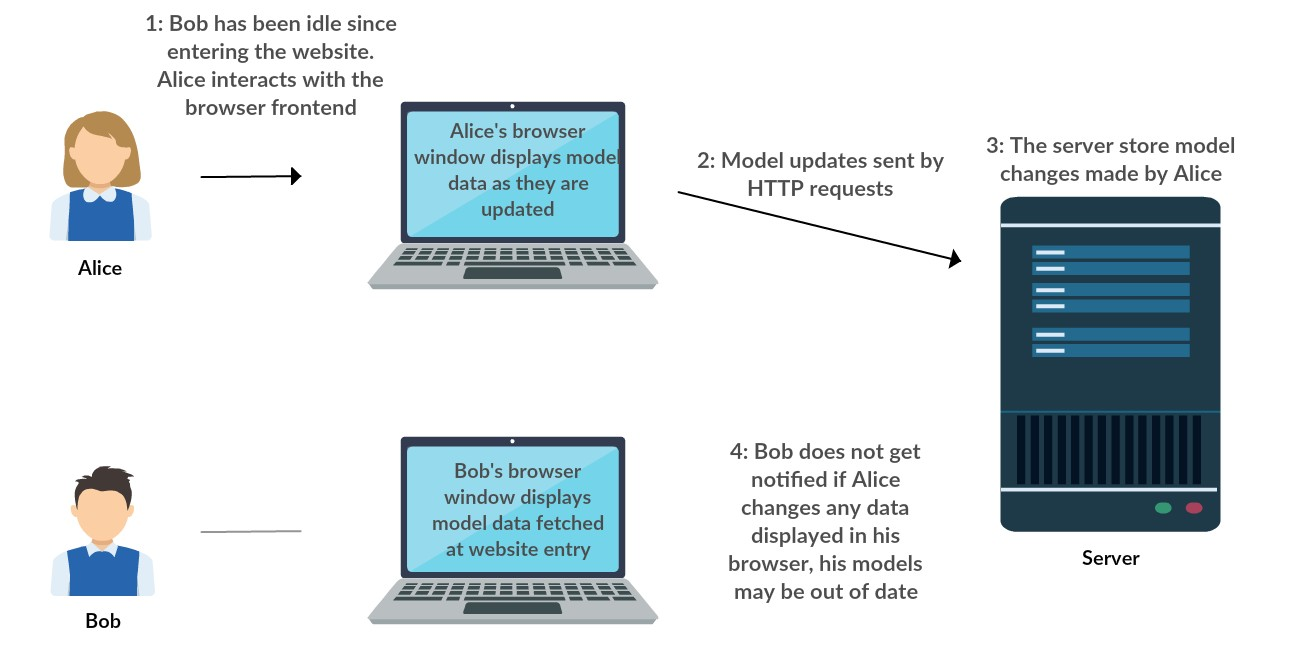
\includegraphics[width=1\textwidth]{figs/update_problem.jpg}
    \caption{Example of updating models without model change notifications}
    \label{fig:update-problem}
\end{sidewaysfigure}

Many websites requires to share data between multiple clients and dynamically notify clients if there are changes to the data. As an example in the \gls{cmb} system, it would be nice if the frontend interface dynamically updated as a user's submission finished running at the backend. In the old system before the improvements, the user had to manually refresh by clicking at a refresh button provided by the user interface or manually refresh the webpage. However, this section presents a technology which has been introduced in the new version of the system in order to dynamically update data relevant for multiple clients. \\

Socket.io \cite{SOCKETIO} is an \gls{api} for enabling real time communication between the server and connected clients. The \gls{api} was first made as Javascript library, but many open source projects have developed modules for other programming languages integrating the Socket.io \gls{api}. One benefit of the \gls{api} is that it works as a wrapper around a set of real time communication protocols to enable support for different browsers, which means that the framework can automatically detect the protocol supported by a client and use that information to select the best fitted communication protocol. \\

Rohit Rai states the communication protocols supported by the Socket.io \gls{api} \cite{Rai2013}. Figure \ref{fig:cmb-protocols} shows the communication protocols enabled in the new version of \gls{cmb}. The WebSocket protocol \cite{a:Fette2011}, shown in Figure \ref{fig:websocket}, has become more popular since its introduction in 2011 and is now supported by the most popular browsers. The protocol is a bit different from the well known HTTP protocol, as there is a persistent connection, or socket, between the client and the server as long as both entities are connected to the socket. The socket connection is closed if the client closes the browser window or the server goes down, or if the code explicitly indicates to close the socket. WebSockets enables easy two-way communication by letting two entities emit (read: send) messages back and forth on the socket connection, and respond differently depending on the type of message emitted on the socket. \\

Polling and long-polling both use the HTTP protocol and may seem similar at first glance. However, in long-polling, the server keeps the connection between the two entities open until there is an update to the requested data as shown in Figure \ref{fig:long-polling}. In polling, as shown in Figure \ref{fig:polling}, the client continuously requests data with some constant delay between each request, while the server respond on each request with the data currently stored at the server. Independent of the protocol, we can think of the connection between the server and client(s) and think of it as a "socket". \\

\begin{figure}
    \centering
    \begin{subfigure}[b]{1.0\textwidth}
        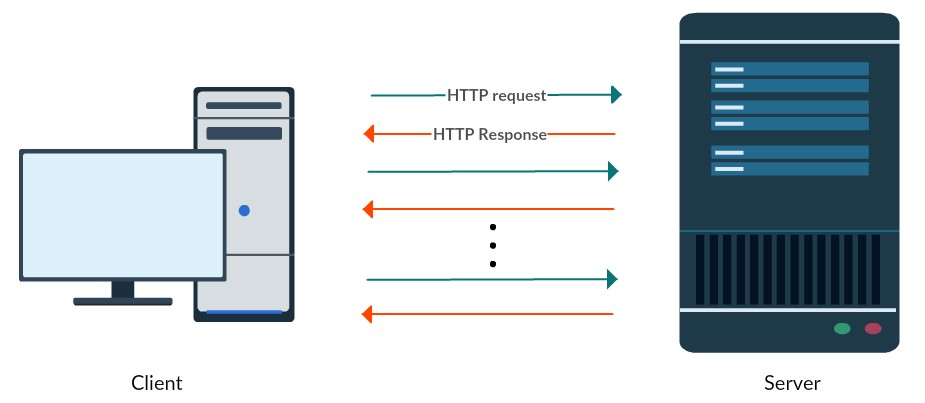
\includegraphics[width=\textwidth]{figs/polling.jpg}
        \caption{Polling: The client sends a series of HTTP request and the server responds on each request.}
        \label{fig:polling}
    \end{subfigure}
    ~ %add desired spacing between images, e. g. ~, \quad, \qquad, \hfill etc.
    %(or a blank line to force the subfigure onto a new line)
    \begin{subfigure}[b]{1.0\textwidth}
        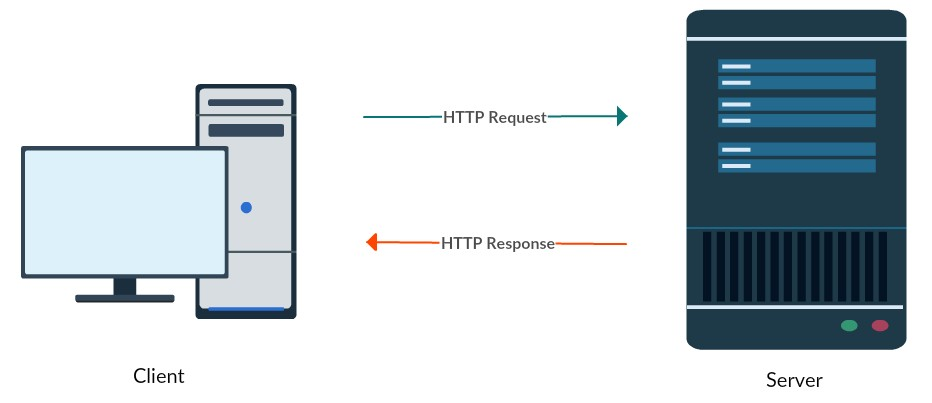
\includegraphics[width=\textwidth]{figs/long_polling.jpg}
        \caption{Long-polling: The client sends an HTTP request to fetch new data, the server holds the connection open until the requested data is updated.}
        \label{fig:long-polling}
    \end{subfigure}
    \begin{subfigure}[b]{1.0\textwidth}
        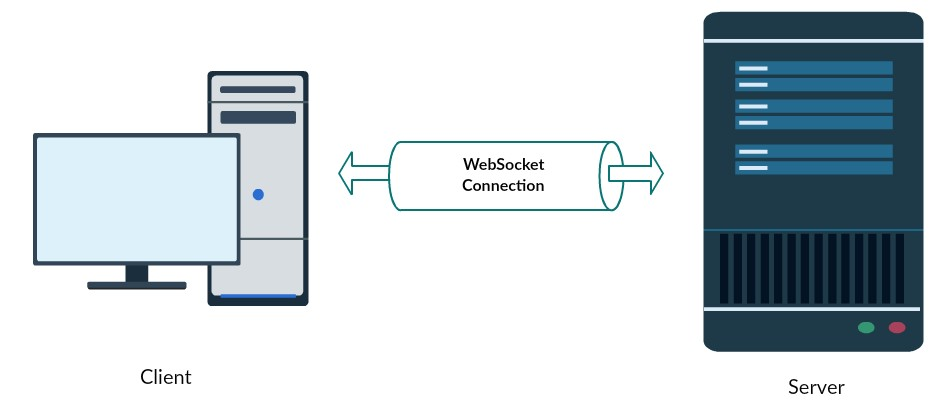
\includegraphics[width=\textwidth]{figs/websocket.jpg}
        \caption{WebSocket protocol: a two-way connection tunnel open throughout the whole client session. TCP is used as a transport protocol.}
        \label{fig:websocket}
    \end{subfigure}
    \caption{\gls{cmb} Socket.io communication protocols}\label{fig:cmb-protocols}
\end{figure}

Each socket can be "\textit{namespaced}" into separate communication channels within an application. A namespace can be viewed as a endpoint or network path, for example in the new \gls{cmb} prototype the namespace \textit{/cmb} is used as default namespace to emit messages between the client and the server. Every client initiating a socket on the namespace receives all messages emitted to the namespace, which makes it easy to share information between the server and clients connected to the namespace. \\

Each namespace can also define a set of \textit{rooms}, which can be viewed as sub-channels of a given namespace. A client needs to explicitly join a room to receive the messages emitted in a given sub-channel. Figure \ref{fig:namespaces-and-rooms} illustrates the concept. Each message emitted to the namespace \textit{/cmb} are received by both client one and two. Client three will only receive those messages emitted to the namespace \textit{/test}. If a message are emitted to room one within the \textit{/cmb} namespace, only client one will receive the message. \\

Socket.io also lets the programmer define \textit{events}, which can be emitted between the server and connected clients. Table \ref{tab:cmb-socketio-events} shows the events currently defined for the \gls{cmb}, and the actions taken either by the server or client depending on which enitity that emitted the event. The two below sub-sections describes the technologies used by the server and frontend in order to support real time communication with Socket.io.

\begin{table}[t!]
    \centering
    \begin{tabular}{ | c | c | c | p{3.5cm} | }
    \hline
    \textbf{Event Name} & \textbf{Emitted by} & \textbf{Received by} & \textbf{Action}\\
    \hline
    \textit{join-problem} & Client(s) & Server & Server adds the client to the problem room specified in the emitted message. \\ \hline
    \textit{leave-problem} & Client(s) & Server & Server removes the client from the problem room specified in the emitted message. \\ \hline
    \textit{submission-deleted} & Server & Client(s) & Client fetches updated submission data from the server. \\ \hline
    \textit{submission-enqueued} & Server & Client(s) & Client displays a message in the browser window, notifying about queue size and information present in the emitted message. \\ \hline
    \textit{submission-dequeued} & Server & Client(s) & Client displays a message in the browser window, notifying about queue size and information present in the emitted message. \\ \hline
    \textit{submission-finished} & Server & Client(s) & Client loads own submissions as well as possible updates to the highscore list. \\ \hline
    \end{tabular}
    \caption[\gls{cmb} Socket.io events and corresponding actions]{\gls{cmb} Socket.io events and corresponding actions. Each submission event is sent within a room which simply is the database id of a given problem. Since we have one room per problem, we know that all submission events within a room has information about submissions made to a given problem.}
    \label{tab:cmb-socketio-events}
\end{table}

\begin{figure}
    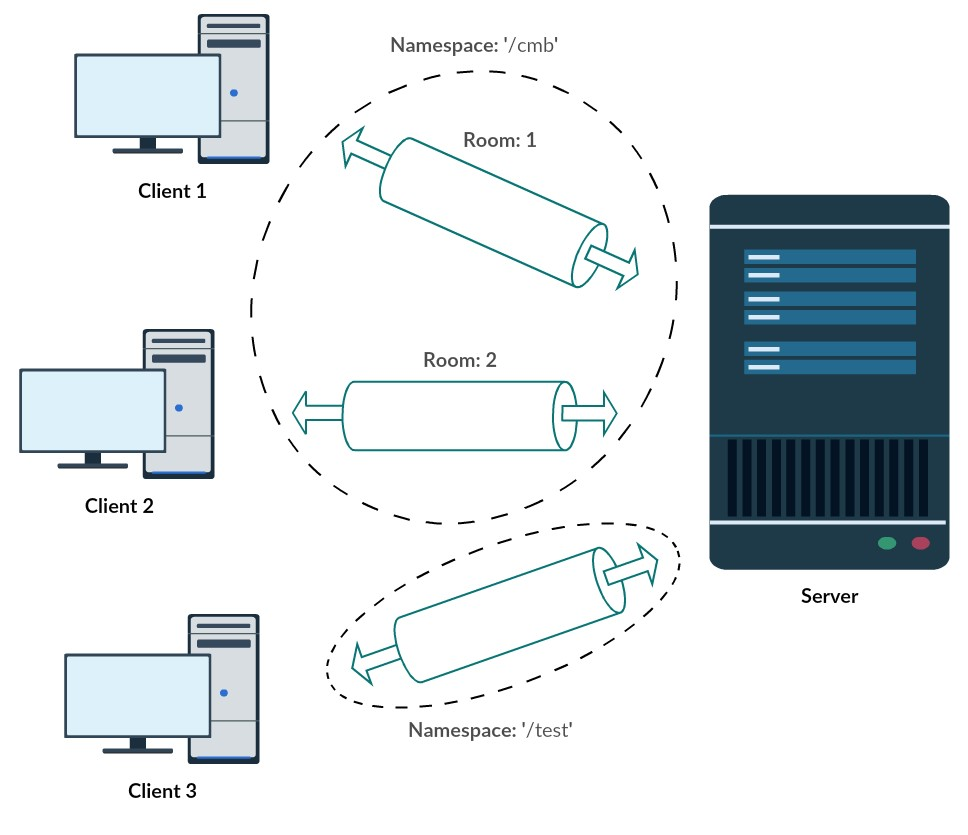
\includegraphics[width=1.0\textwidth]{figs/namespaces_and_rooms.jpg}
    \caption[Socketio namespaces and rooms in the \gls{cmb} system]{Socketio namespaces and rooms in the \gls{cmb} system. }
    \label{fig:namespaces-and-rooms}
\end{figure}

\subsection{Frontend Technology}
The frontend uses the client Socket.io library \cite{SOCKETIO} through a existing Angular component called \texttt{angular-socket-io} provided by Brian Ford \cite{ANGULARSOCKETIO}. The component is used to define a Angular \textit{factory}, which is simply gathers and structures the setup of Socket.io in the client in a single service. The defined factory can then be used by other components in the Angular app, by marking components as dependent of the Socket.io factory. \\

The problem-controller uses the defined Socket.io factory. The controller is associated with the problem-view, which describes a problem provided by \gls{cmb} as well as submissions made by users. More about the view + explanation with table.

\subsection{Server Technology}
The Python module Flask-SocketIO \cite{FLASKSOCKETIO} enables Flask applications to use the SocketIO \gls{api}. In addition, the modules gevent \cite{GEVENT} and gevent-websocket \cite{GEVENTWEBSOCKET} is installed in combination with the Socket.io module to enable the use of the WebSocket protocol. Gevent is a coroutine based networking library providing a high-level synchronous API on top of a asynchronous webserver. Asynchronous coroutines is used to handle multiple concurrent requests from multiple clients, and is required by the Flask-SocketIO module to support the WebSocket transport. \\

To fully support the WebSocket protocol Gunicorn also needs to make use a custom gevent worker supporting the WebSocket protocol. As stated by Miguel Grinberg on the Flask-Socketio documentation website, Gunicorn can only enable one worker due to limitations in the implemented load balancing algorithm. The Gunicorn load balancing algorithm cannot simply handle multiple workers and persistent WebSockets connections, which limits us to one worker per server. However, the worker uses coroutines to handle multiple concurrent requests as stated above. The gevent worker is enabled on the development server of \gls{cmb}, which also required some changes to the Nginx setup to fully support the WebSocket protocol. Appendix \ref{apdx:setup} describes setup information necessary to setup servers with Gunicorn and Nginx, while section \ref{sec:eval-tech} discusses pros and cons with selected technologies as well as presenting alternatives to the selected technology stack.

\section{Frontend}
\label{sec:impr-frontend}
\subsection{Bug Fixes}
Upload fixes in frontend
Sorting bug

\subsection{Views and Feedback}
Spinners + better error messages. Symbols added for usability. Bulletin board to display administrator messages. Colored feedback messages.

\subsection{Group Functionality Improvements}
JSON stat file download. Gathered group functionality.

\section{Server}
\label{sec:impr-server}
\subsection{Database Management System Updates}
The old version of \gls{cmb} used SQLite \cite{SQLITE} as \gls{dbms} at both the development and production server. SQLite is a lightweight \gls{dbms} which requires minimal configuration before use and is therefore popular to use during automatic unit testing, which also is done in the \gls{cmb} system. The initial goal were to improve, and thereby possibly change, the \gls{dbms} into a more sophisticated system. However, during the Spring the \gls{cmb} team found it uneccassery to change the \gls{dbms} of performance reasons and we found it more important to extend the system with new features. \\

Unrelated to the performance reasons, a new \gls{dbms} was wanted by the \gls{cmb} team and the IDI Department. We therefore changed the \gls{dbms} to MySQL due to its usage in other applications developed at the IDI Department. IDI provided the databases used by the system, and we also gained access to a database adminstrator interface available at \url{https://phpmyadmin.idi.ntnu.no/}. SQLAlchemy made the switch onto the new \gls{dbms} easy as it has a predefined MySQL adapter, and had no problems in setting up the new databases for our development and production servers. Further, Flask-Migrate \cite{FLASKMIGRATE}, used for database \textit{migrations}\footnote{Database magration is the task of managing versions of a database schema without altering previously stored database content.}, also worked without any changes in configuration. \\

A complete database dump were made from the SQLite databases. All SQL \texttt{INSERT} statements in the database dump were extracted and executed against the new development and production databases, to move all previously stored data in the SQLite databases over to the MySQL databases. The actions were performed with a combination of terminal commands and the database admin interface provided by IDI. MySQL and SQLAlchemy has not had any performance issues in the IDI Department, so the system uses the standard MySQL adapter provided by SQLALchemy. Implementing and enabling non-blocking database access has been added back to the backlog found in Appendix \ref{apdx:backlog} as a performance improvement.

\subsection{Database Schema Updates}
The updated database schema is shown in Figure \ref{}. The Submissions-table have been updated with two new fields. The ``detailed state''-field was added to provide more information about a run to the user. In the current improved system, it contains a detailed string about a submissions state as it returns from the backend as explained in section \ref{sec:impr-backend}. The field can be modified in the future to store \gls{json} instead of simple text, if more information about a submission becomes available when executing code on the backend. \textit{Future developers should stribe to always keep users up-to-date with the state of their submissions}, and the new field aims to enable such feedback as explained in the section \ref{sec:impr-frontend} above. \\

A Bulletin-table were added to enable administrators to notify users about news and system messages. Bulletins has a field called \textit{valid\_until} which indicates until which date a given bulletin is valid, and the field is used to select the valid bulletins as explained in the below sub-section and is also displayed in the frontend as explained in section \ref{sec:impr-frontend} above. \\

Cascading deletes has also been added between the Submission- and Run-tables. This ensures that all rows in the Run-table associated with a Submission-row gets deleted upon delition of a submission, which ensures that there are no dangling rows in the Run-table and the database is left in a consistent state after deleting submissions. This is particularly important as both administrators and users are able to delete submissions.

\subsection{Routes}
The routes that has been updated or added to the \gls{rest}ful \gls{api} is listed in Table \ref{tab:cmb-updated-routes}. The table does not include changes made to \gls{api} routes due to the implementation of the real time update improvement explained in section \ref{sec:real-time}, as the improvements does not change the internal logic of the original routes and has only added code to emit events to enable real-time updates of possible connected clients. \\

Add example from postman + image.

\begin{table}[h!]
    \centering
    \begin{tabular}{ | c | c | p{4cm} | }
    \hline
    \textbf{\gls{api} Route} & \textbf{Method} & \textbf{Description} \\
    \hline
    \textit{/api/submission/$<$int:sub\_id$>$} & DELETE & If the submission with the given \texttt{id} exists and have been created by the current logged in user, the submission is deleted from the database as well as the file system. Requires login.\\ \hline
    \textit{/api/group/$<$int:group\_id$>$} & GET & Fetches information about a group by \texttt{id} depending on login status. If the user is not logged in, only public groups can be fetched. However, if the user is logged in, the user can also request information about private groups. If the query parameter \texttt{with-submissions} is set equal to 1, submissions made from group members is included in the response if the user is either a group member or leader. The response for leaders also include those submissions set to be unvisible. \\ \hline
    \textit{/api/bulletins} & GET & Returns all created bulletins. \\ \hline
    \textit{/api/bulletins/active} & GET & Returns all bulletins currently active. \\ \hline
    \end{tabular}
    \caption[\gls{cmb} API route updates with responses]{\gls{cmb} API route updates with responses. The routes listed shows the substring necessary to query the \gls{api}, and need to be combined with the \textit{path} of the server providing the \gls{api}. For example to delete a submission with \texttt{id} 1 from the development server \gls{api}, a delete request needs to be made against \url{http://climb-dev.idi.ntnu.no/api/submission/1}.}
    \label{tab:cmb-updated-routes}
\end{table}

\subsection{Admin Interface}
Several new problems have been added to the system during the Spring semester. Most problems were added due to a master thesis of two students, assessing the \gls{cmb} system's suitability for conducting digital exams in the course TDT4102 Procedural and Object-Oriented Programming \cite{TDT4102}. However, during the Spring we had a lot of trouble making the newly added problems solvable, as some submissions locked the backend infinetely. It turned out that some of the administrators had uploaded input and answer files with CR/LF (DOS) line endings, which locked the checker program during parsing of the input and answer files. The checker program locked itself, as the backend and server is Unix based systems and uses Unix line endings (LF). \\

The bug is removed in the new admin interface. When uploading files to the server, the files are automatically converted into Unix files with LF line endings. This is done by running all input and answer files through the \texttt{vim} \cite{VIM} command \texttt{vim + "argdo set ff=unix | update" +wqa ./*.txt} in the directory containing the problem files. The checker source file is not run through the command as the g++ compiler handles both Unix and DOS filetypes. \\

In addition some errors occured when administrators tried to remove locked submissions in the database through the admin interface. Due to lack of training, it often left the database and the server file system in a inconsistent state. As explained above, cascading delete were added between the \texttt{Run} and \texttt{Submission} tables to partially solve the problem, but the files associated with a submission would still remain in the server file system and had to be removed manually. However, deletion of submission files were often forgotten and it caused filename conflicts if the user re-submitted zip files with equal folder and file names as a previous submission.\footnote{A suggested future improvement is presented in section \ref{sec:future-work}, which is based upon storing submission files by the uniquely generated database id instead of using user defined folder and file names.}\\

The Flask-Admin \cite{FLASKADMIN} procedure \texttt{on\_model\_delete} solves the above inconsistency problem. It has been added to handle when submissions are deleted from the database, and takes care of removing all files in the server file system assoociated with a deleted submission. However, it is still possible to leave the database in a inconsistent state if one do not use the admin interface to delete database content. If other tools than the Flask-Admin module are to be used in the future to handle database, SQLALchemy provides event listeners which can be used instead of the above mentioned procedure. As the \gls{cmb} team currently uses the admin interface to handle database content, the \texttt{on\_model\_delete} procedure in the Flask-Admin interface is used. \\

Bulletin board admin view + images.

\section{Backend}
\label{sec:impr-backend}
There have been some small changes in the backend code. The \gls{cmb} team discovered that there were no timeout when running the small correctness test, which could potentially lock the backend if the submitted code contained infinite loops. Locking the backend should not be acceptable under any condition, and the Unix program \texttt{timeout} \cite{TIMEOUT} is therefore used as during the big correctness test to kill the submitted program after some time if it stalls to long. Since the small input set is much smaller than the big correctness test, it is currently set to a third of the timeout of the big correctness or 30 seconds. \\

The \gls{json} returned by the backend is also slightly changed. A ``state'' field were added to better track the state of the program as it executes on the backend, especially if there is an error during execution. The field is currently used as input to the ``detailed state'' database field as described above, which is further used in the frontend to specialize the feedback given to the user if there is an error during execution of the program. Currently, the field is a simple string describing the state of the submitted program when the backend are done executing. A quick further discussion of the field and its potential are described in section \ref{sec:eval-tech}.

\section{Improvement Proposals}

\subsection{Stability Test}

\subsection{How-To Page and About Page}

\subsection{Adding Problems}

\subsection{Discussion Forum}

%!TEX root=../main.tex
\chapter{User and System Testing}
\label{ch:testing}
This chapter will explain the testing of usability of the developed system. \Cref{sec:cont-user-testing} starts off with a brief presentation of the small continuous user testing, which was concucted during development of new features. Further, \Cref{sec:user-testing} presents the motivation, methodology, and results from a large scale user test conducted April 18th, and the results are compared to results gathered and presented in the specialization report. The chapter ends with a presentation of system unit test coverage in \Cref{sec:system-unit-tests}. This chapter covers the following objectives presented in \Cref{sec:ps-inter}:
\begin{itemize}
  \item Conduct a user-experiment to evaluate system usability, i.e objective \texttt{U3}.
\end{itemize}

\section{Continuous User Testing}
\label{sec:cont-user-testing}
ISO 13407 part 210 \cite{iso1999HCD} describes the practice of user-centered design. To achieve high usability in a system, it is important to involve end-users early in the design process, as they might have other requirements to the system compared to system designers and developers. Figure \ref{fig:user-centered-design} summarizes the iterative steps of the process. First we have an idea and specify the usage of the idea in the system, before specifying requirements set by users. Then we develop a design prototype, and evaluate whether the design meets user requirements. If the new design meets user requirements it is integrated into the system, but if it is not accepted, we go back to the stage in the user-centered design process, which needs revision or modifications. \\

\begin{figure}
  \centering
  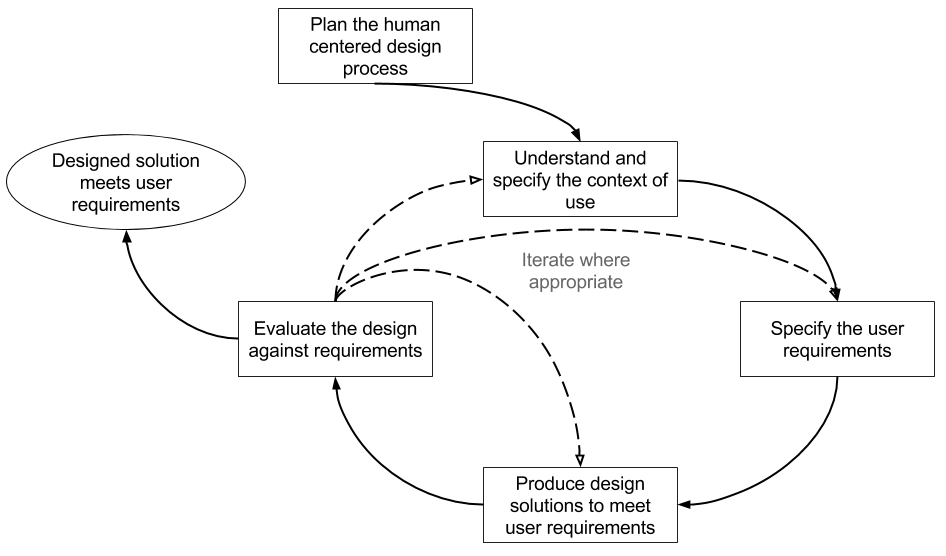
\includegraphics[width=1.0\textwidth]{figs/iterative-design-process.png}
  \caption[User-centered design process]{User-centered design process (adapted from: \cite{iso1999HCD}).}
  \label{fig:user-centered-design}
\end{figure}

System development during the Spring has followed a similar process as the user-centered design approach described above. Requirements were specified by the \gls{cmb} team, and a design prototype was developed and tested on possible end-users. Users were asked if they liked the new feature and they were also presented with the old user interface for comparison. If the test users liked the new feature it was accepted, otherwise it was further developed or revised until accepted. \\

Test users included supervisors, project team members, and student acquaintances. Both the admin interface and user interface features were tested according to the above process. Future developers are advised to follow a user-centered design approach such as the Lean Startup methodology \cite{ries2011}, which has become fairly popular during the last few years.

%\subsection{Admin Interface Assessment}
%Some system administrators were also asked to assess the usability of the improved admin interface. The admin interface usability assessment was not a part of the user test, as the user test focused on testing the frontend interface used by normal users. We also have an restrictive amount of system administrators which has been trained in how to use the interface, which makes a test of the admin interface on a wast amount of participants unnecessary.


%\subsection{Validity}
%\paragraph*{Admin Interface Assessment} \hfill \\
%The number of admin users are small and might not be statistically significant. However, since the number of admin users is small and will stay small for some time in the future, it is important that the few admin users we have like the new admin interface improvements. Consequently, the assessment will likely be affected with experience from and observations done in the old admin interface. To improve the credability of the results one could also include testing of the admin interface in the optimal user test described above. However, this would make the user test more extensive and harder to execute, and would require a lot of administrative work.

\section{User Experiment}
\label{sec:user-testing}

\subsection{Motivation}
A user test was performed in the specialization project and the project report was delivered in December 2015 as mentioned in \Cref{subsec:related-proj}. The \gls{cmb} system was one of three tools used by the students in mandatory assignments, where the \gls{cmb} system mainly was used for testing the system on more users then previously attempted by Follan and Støa \cite{mt:T&S}. The course assignments cover various topics and methods of producing parallel code in C++, like OpenMP, NEON, MPI and CUDA, and is about 25\% of the workload during the semester for the average student. The TDT4200 course staff added in total five programming problems to \gls{cmb}, which were solved by most students, and the system received a lot of submissions during the semester. \\

During November of 2015 a total of 37 students delivered an optional questionnaire, which included some questions about the \gls{cmb} system. In addition to the questionnaire, some feedback on the system was gathered during the last lecture of the course late in November. The feedback was mainly focused on usability aspects of the system, which helped the \gls{cmb} project team to discover bugs, and to setup and prioritize features to implement next. The prioritized list generated a backlog, which was used as a motivation when constructing the objectives presented in \Cref{sec:ps-inter}. \\

As this thesis potentially has improved system usability, it is interesting to conduct a user study to compare the usability of the two system versions. As mentioned in \Cref{sec:cmb}, the system developed by Follan and Støa will be referred to as system version one, while the updated system presented in \Cref{ch:improvements} will be referred to as system version two in the below discussion. As mentioned in \Cref{sec:usability-def}, usability is a broad term and this thesis has contributed mainly against improving efficiency, learnability, and satisfaction of users as discussed in \Cref{ch:design} and implemented in \Cref{ch:improvements}. The above observation makes it interesting to test the following hypothesis:

\paragraph*{Hypothesis 1:} The usability, in terms of either efficiency, learnability, or user satisfaction, is higher in system version two compared to system version one. \hfill \\

%Further, it is interesting to investigate if the overall usability of the system has increased in the \gls{cmb} system version two i.e:

%\paragraph*{Hypothesis 2:} The overall usability of system version two is higher compared to system version one. \hfill \\

\subsection{Methodology}
\label{sub-sec:user-testing-methodology}
The user test was conducted April 18th this Spring and assesses the system improvements presented in \Cref{ch:improvements} with focus on usability. The goal of this second test is to further improve the results received from the specialization project user test also called user test one. The second test required an interest in programming and programming experience from the participants, but no prior knowledge of C or C++ or any parallel programming libraries were set as a requirement to participate in the test. \\

The weak requirements were set since there was generally low interest from students in participating in the test. The low interest in the test is most likely due to bad timing, as many students have several assignment deliverables before their last lectures in mid April. Furthermore, attracting students or others to participate in a user test for a master thesis is generally hard if the test takes several hours. \textit{As the focus of this test was to test the usability of the system, it should be sufficient for participants to have general knowledge and interest in programming to assess system usability}. \\

The user test described a set of tasks to be completed by each participant. Since we are comparing the two system versions, the test does not assess the new features implemented and is assumed covered by \Cref{sec:cont-user-testing}. Appendix \ref{apdx:usertest} presents the tasks executed by every participant during the test, along with a questionnaire each participant was to complete before finishing the user test. \\

Nearly all participants conducted the test simultaneously in a lecture hall to simulate the heavy submission traffic we experienced before assignment deadlines in TDT4200. A couple of participants started the user test late or participated a couple of days after the official user test, to simulate the students in TDT4200 that experienced little or no traffic. Participants were informed that questions related to how to complete a task would not be answered during the test and that tasks should be completed individually. They were also informed that they could abort the test at any time. \\

\begin{table}
    \centering
    \begin{tabular}{ | l | p{6cm} |}
    \hline
    \textbf{Problem Name} & \textbf{Problem Description Summary} \\ \hline
    Hello World & Print out "Hello World!"". \\ \hline
    Digits & \textit{T} test cases are given as input, each test case describing the range between two numbers \textit{N} and \textit{M}. For each test case, output the number of zeroes present in all the numbers in the range [\textit{N}, \textit{M}]. \\ \hline
    Prime Number & For every number in the input, output if the number is a prime. \\ \hline
    WERTYU & For every encrypted input string, decrypt it and output the decrypted string. Hint: The input strings are encrypted with a QWERTY keyboard shifted one character to the right. \\ \hline
    Reverse String & For every input string output the reversed string. \\
    \hline
    \end{tabular}
    \caption{Available solvable problems during user test.}
    \label{tab:avail-prob}
\end{table}

The most time-consuming task the participants had to complete was to submit code to one of the problems presented in Table \ref{tab:avail-prob}. Submitting code to problems is the core of the \gls{oj} and the process of uploading and running submissions was the most common procedure done by TDT4200 students. The procedure and aspects related to submissions was also mentioned the most times in feedback given by the TDT4200 students, and was therefore chosen as one of the main tasks to perform in this user test. Before starting the user test, the participants were also notified to comment extensively on the procedure when filling out the survey. \\

The participants who were unfamiliar with C and C++ were given five different source files to the ``Prime Number''-problem, which they were to submit to the system. The thought behind handing out source files, was to simulate that the participants made a number of tries before arriving at the correct solution. The ``Prime Number''-problem was chosen as it is of medium to easy difficulty. Participants who knew either C or C++ were also motivated to try to solve more than one problem if they arrived at a solution quickly, in order to extensively test the procedure of uploading and running submissions. Other tasks executed by participants included sign-up, login, viewing submissions and highscore lists, joining groups, creating and administering groups, and changing user e-mail and password. \\

The questionnaire found in Appendix \ref{apdx:usertest} contains the same questions about the \gls{cmb} system presented in the questionnaire given to the students in TDT4200. The questionnaire is, as mentioned in the Specialization project report, inspired by a typical Likert scale form developed by IBM\footnote{See: \url{http://garyperlman.com/quest/quest.cgi}.} and complemented with textually based questions. To compare the results of the two questionnaires, it is important that they cover the same aspects, and all questions developed in the specialization project are therefore reused in the questionnaire handed out in this user study. In addition, a couple of extra multiple choice questions were added to the questionnaire of this test for the sake of clarity. \\

Likert scale questions are often used in usability assessment of software systems. In this test, the number of Likert scale alternatives is set to five per question. Each row in Table \ref{tab:likert-scale} shows the possible alternatives for a given question type, as well as each alternative's corresponding score ranged from one to five. The answers to Likert scale values of the two user tests are then compared using statistical analysis as explained in \Cref{sub-sec:user-test-statistics}. To make it easier for participants to describe their thoughts about system features, the textually based questions are provided in the questionnaire and are further used as qualitative support when discussing the user study results.

\begin{table}[t!]
    \centering
    \begin{tabular}{ | c | p{1.5cm} | p{1.5cm} | p{1.5cm} | p{1.5cm} | p{1.5cm} |}
    \hline
    \multirow{2}{*}{\textbf{Question Type}} & \multicolumn{5}{ c| }{\textbf{Likert Score Range}} \\ \cline{2-6}
      & 1 & 2 & 3 & 4 & 5 \\ \cline{1-6}
    A & Very poor & Poor & Neutral & Good & Very good \\ \hline
    B & Strongly disagree & Disagree & Neither agree or disagree & Agree & Strongly agree \\ \hline
    C & Very hard & Hard & Neutral & Easy & Very easy \\ \hline
    D & Not satisfied at all & A~little bit~satisfied & Neutral & Satisfied & Very satisfied \\ \hline
    \end{tabular}
    \caption{Likert scale alternatives on question type.}
    \label{tab:likert-scale}
\end{table}

\subsection{Statistical Analysis}
\label{sub-sec:user-test-statistics}
The tool Gnumeric \cite{GNUMERIC} is used for statistical data analysis comparison of the multiple choice results of the two user tests. The results are reproducible using the pie charts and number of participants of each user test found in Appendix \ref{apdx:usertest}. Each multiple choice answer from both tests is translated into the corresponding Likert scale value, and values of matching questions between the two user tests are then compared. To simplify the discussion of results and validity, the user test conducted as part of the Specialization project will be referred to as user test one or T1 and the user test conducted in this thesis will be referred to as user test two or T2. \\

An F-test \cite{moore2007} is conducted to determine whether the compared data set variances can be considered equal. The F-test calculates a P-value, which is a measurement of how extreme the results of a given test are relative to the underlying statistical model. The P-value is compared to a defined significance level, and variances are considered equal if the P-value is less than the decided significance level or unequal if the P-value is bigger than significance level. The result can also be formulated as keeping the null hypothesis ($H_0$), while the opposite situation is referred to as rejecting the null hypothesis and accepting the alternative hypothesis ($H_1$). \\

A T-test \cite{walpole1993} is performed on each question to determine whether two user tests have significantly different means. The T-test can be executed either assuming equal or unequal variances, and the result of the F-test determines which version of the T-test to execute. The T-test also outputs a P-value, which is used in the same way as explained in the above paragraph. \\

The statistical analysis in this thesis assumes a significance level ($\alpha$) of 5\%. Furthermore, the null hypothesis ($H_0$) for the T-test assumes equal means of the two datasets, while the alternative hypothesis ($H_1$) is set depending on if we are conducting either a one-tailed or two-tailed T-test. Equation \ref{eq:h1-t-test} shows the possible alternative hypothesis for the T-test, where $\mu_{1}$ and $\mu_{2}$ are the means for user test one and two respectively. In this thesis we use the one-tailed alternative hypothesis, as we want to obtain stronger results for system version two.

\begin{equation} \label{eq:h1-t-test}
   H_1 =
    \begin{cases}
        \mu_{2} > \mu_{1} & \quad \text{if one-tailed test}\\
        \mu_{1} \neq \mu_{2} & \quad \text{if two-tailed test}\\
    \end{cases}
\end{equation}

If the T-test indicates a significant difference between the two user groups further analysis is needed. If so, an Anderson-Darling test \cite{razali2011} is performed to check the normality of the data sets, as normality is often a requirement for a valid T-test. However, if the normality check fails, the non-parametric \gls{wmw} test \cite{hodges2005} is performed on each of the question groups accepted by the T-test. The test is used to support the conclusion of the T-test, as non-parametric tests are often used when the compared data sets are non-normally distributed. \\

The statistical effect-size is also reported and used when discussing the results. The effect-size is meant by the statistical \textit{strength} of a result, and will be important in our discussion of the multiple choice results. The reported effect-size metrics used is Cohen's d, Hedge's g, and Pearson's r \cite{cumming2013}.\footnote{Calculated with this tool: \url{http://www.polyu.edu.hk/mm/effectsizefaqs/calculator/calculator.html}.} Cohen's d is often used as effect size to measure the strength of a T-test, as well as Pearson's r which is a well known effect-size metric. Hedge's g is also included in the results, as it is more accurate than Cohen's d with small sample sizes. Table \ref{tab:effect-size} reports the strength scale for each of the used effect-size metrics, and a conclusion from a test is considered stronger the higher effect-size reported. \\

Cohen's d and Hedge's g are also used to calculate the statistical \textit{power} of a conclusion. Statistical power is the probability of correctly rejecting $H_0$ when $H_1$ is true, and is important when discussing threats against validity to be sure that we have enough respondents to draw valid conclusions. Statistical power of the T-test is calculated using the Real Statistics Resource Pack in Microsoft Excel \cite{RSRP}.

\begin{table}[t!]
    \centering
    \begin{tabular}{ | c | c | c | c |}
    \hline
    \textbf{Effect size} & \textbf{Pearson's r} & \textbf{Cohen's d} & \textbf{Hedge's g} \\ \hline
    Small & 0.1 & 0.2 & 0.2 \\ \hline
    Medium & 0.3 & 0.5 & 0.5 \\ \hline
    Large & 0.5 & 0.8 & 0.8 \\ \hline
    \end{tabular}
    \caption{Effect sizes and corresponding metric values.}
    \label{tab:effect-size}
\end{table}

\subsection{Results and Evaluation}
\label{sub-sec:user-testing-results}
There were in total 21 participants in the second user test. Table \ref{tab:label-to-title} shows a mapping between question titles and labels, which makes it easier to refer to the questions in the below discussion. As mentioned, there were a total of 37 TDT4200 students providing feedback in the optional questionnaire given during the Autumn semester. The pie-charts and a summary of textually based feedback for both the user test one and two can be found in Appendix \ref{apdx:usertest}. All statistical test results reported in tables are rounded to three decimal places if applicable, that is, results are not rounded if it changes the outcome of the below discussions. \\

Table \ref{tab:results-tests-all} shows the means and variances of the user test one and two responses for each Likert scale question in common for the two user tests. The table also include F-test P-values and the conclusion of the F-test compared to the significance level, which determines to either assume equal or unequal variances when performing the T-test. The T-test P-value is also reported, and is used to determine if a rejection of null hypothesis is needed. \\

The three questions \texttt{A3}, \texttt{D1}, and \texttt{A4} should reject $H_0$ as indicated by the T-test results in Table \ref{tab:results-tests-all}. However, none of the data sets are normally distributed according to the Anderson-Darling test. Subsequently, a \gls{wmw}-test is conducted to support the conclusion of the T-test. Table \ref{tab:significant-results} reports the resulting P-value of the \gls{wmw}-test, as well as effect-sizes and power calculations. \\

\begin{table}[t!]
    \centering
    \begin{tabular}{ | c | p{9cm} |}
    \hline
    \textbf{Label} & \textbf{Question Title} \\ \hline
    \texttt{O1} & ``What year of study are you in?'' \\ \hline
    \texttt{O2} & ``Which of the following best describes your study programme?''  \\ \hline
    \texttt{A1} & ``How would you rate the Climbing Mont Blanc system in general?'' \\ \hline
    \texttt{B1} & ``It was easy to use the system?'' \\ \hline
    \texttt{A2} & ``How would you rate the usability of the Climbing Mont Blanc system?'' \\ \hline
    \texttt{C1} & ``Was it difficult to learn how to use the Climbing Mont Blanc system?'' \\ \hline
    \texttt{A3} & ``How would you rate the design of the Climbing Mont Blanc user interface?'' \\ \hline
    \texttt{C2} & ``How would you rate the process uploading and running a program?'' \\ \hline
    \texttt{D1} & ``How satisfied are you with the feedback given by the Climbing Mont Blanc system?'' \\ \hline
    \texttt{B2} & ``The feedback given by the system is clear and helpful?'' \\ \hline
    \texttt{A4} & ``How would you rate the information on the HowTo-page?'' \\ \hline
    \end{tabular}
    \caption[Label to question title mapping]{Label to question title mapping: Labels are created according to Table \ref{tab:likert-scale}. Questions marked \texttt{O} are meant as other questions not within the five point Likert scale range.}
    \label{tab:label-to-title}
\end{table}

The \gls{wmw}-test also indicates significant results as its P-values are lower than $\alpha$. Question \texttt{D1} has the most significant results, as the effect-size is large and the power is high using both Cohen's d and Hedge's g. Using Hedge's g to compute power, we can by a 97.2\% confidence value be certain that we have correctly rejected $H_0$ when $H_1$ is true. We can therefore conclude that users, most probably, are more satisfied with the feedback of system version two. The results reported for question \texttt{B2} in Appendix \ref{apdx:usertest} also indicates that feedback is good, as over 80\% of participants either agree or strongly agree that the feedback given by the system is clear and helpful.  \\

\begin{table}[t!]
    \centering
    \begin{tabular}{|c||c|c||c|c||c|c||c|c||}
      \hline
      \multirow{2}{*}{\textbf{Question}} & \multicolumn{2}{ |c|| }{\textbf{A1}} & \multicolumn{2}{ |c|| }{\textbf{A2}} & \multicolumn{2}{ |c|| }{\textbf{C1}} & \multicolumn{2}{ |c|| }{\textbf{A3}} \\ \cline{2-9}
      &  T1 & T2 & T1 & T2 & T1 & T2 & T1 & T2 \\ \hline
      \textbf{Mean} & 3.676 & 3.857 & 3.730 & 3.809 & 3.919 & 3.905 & 3.730 & 4.143 \\ \hline
      \textbf{Variance} & 0.392 & 0.429 & 0.592 & 0.162 & 0.521 & 0.590 & 0.369 & 0.329 \\ \hline
      \textbf{F P-value} & \multicolumn{2}{c||}{0.396} & \multicolumn{2}{c||}{0.002} & \multicolumn{2}{c||}{0.362} & \multicolumn{2}{c||}{0.400} \\ \hline
      \textbf{Variance} & \multicolumn{2}{c||}{Equal} & \multicolumn{2}{c||}{Unequal} & \multicolumn{2}{c||}{Equal} & \multicolumn{2}{c||}{Equal} \\ \hline
      \textbf{T P-value} & \multicolumn{2}{c||}{0.151} & \multicolumn{2}{c||}{0.303} & \multicolumn{2}{c||}{0.472} & \multicolumn{2}{c||}{0.002}\\ \hline
      \textbf{Reject $H_0$?} & \multicolumn{2}{c||}{No} & \multicolumn{2}{c||}{No} & \multicolumn{2}{c||}{No} & \multicolumn{2}{c||}{Yes}\\ \hline
    \end{tabular} \\[5pt]
    \begin{tabular}{|c||c|c||c|c||c|c||}
      \hline
      \multirow{2}{*}{\textbf{Question}} & \multicolumn{2}{ |c|| }{\textbf{C2}} & \multicolumn{2}{ |c|| }{\textbf{D1}} & \multicolumn{2}{ |c|| }{\textbf{A4}} \\ \cline{2-7}
      &  T1 & T2 & T1 & T2 & T1 & T2 \\ \hline
      \textbf{Mean} & 3.595 & 3.524 & 2.568 & 3.619 & 3.324 & 3.842 \\ \hline
      \textbf{Variance} & 0.970 & 0.762 & 0.919 & 0.947 & 0.892 & 0.474 \\ \hline
      \textbf{F P-value} & \multicolumn{2}{c||}{0.287} & \multicolumn{2}{c||}{0.454} & \multicolumn{2}{c||}{0.060}\\ \hline
      \textbf{Variance} & \multicolumn{2}{c||}{Equal} & \multicolumn{2}{c||}{Equal} & \multicolumn{2}{c||}{Equal} \\ \hline
      \textbf{T P-Value} & \multicolumn{2}{c||}{0.393} & \multicolumn{2}{c||}{$9.6x10^{-5}$} & \multicolumn{2}{c||}{0.022} \\ \hline
      \textbf{Reject $H_0$?} & \multicolumn{2}{c||}{No} & \multicolumn{2}{c||}{Yes} & \multicolumn{2}{c||}{Yes} \\ \hline
    \end{tabular}
    \caption{Mean, variance, F-test, and T-test results.}
    \label{tab:results-tests-all}
\end{table}

The questions \texttt{A3} and \texttt{A4} are also accepted by both the T-test and \gls{wmw}-test. However, their strength in terms of all effect-size metrics indicates medium strength for \texttt{A3} and low to medium strength for \texttt{A4}. The statistical power of question \texttt{A3} and question \texttt{A4} should have been higher for us to draw any valid conclusions. We can only conclude that system version two might have a better user interface design and an improved HowTo-page. \\

The overall usability is good in both system versions. This also corresponds to the conclusion of tests ran against question  \texttt{C1}, and answers to textually based feedback received from both user test one and user test two. There is also generally little overlap in textually based feedback, which indicates that there have been some improvements to usability. Some of the textually based feedback, such as adding language versions and project information to the HowTo-page as proposed in \Cref{sec:impr-proposals}, has already been noted by the \gls{cmb} team and is already listed in the backlog found in Appendix \ref{apdx:backlog}. \\

The textually based questions are as mentioned meant as support for the multiple choice questions. The questions are also important for the future development of the \gls{cmb} prototype. Proposals of new features, such as reporting low-level statistics, allowing uploading multiple files, and updated feedback on placement in the run-queue have been noted by the \gls{cmb} team. \Cref{sec:future-work} presents these features and they have also been added to the backlog in Appendix \ref{apdx:backlog}. \\

Some of the feedback noticed by participants, such as real-time updates of submission placement in the run-queue, was actually in the making shortly before the conduction of the user experiment. As the improvements showed to be more extensive to implement than first thought, they were not implemented. The choice was made as it was little time to develop unit tests and test the implementation before the conduction of the user test, and the features also required changes to backend code which was the domain of another master student. \Cref{ch:evaluation} further discusses the matter. \\

The experiment results indicate that users are more satisfied with version two of the system. Users are from the above study more satisfied with the feedback given by system version two, and there is also a trend towards users being more satisfied with the user interface design and the information displayed on the HowTo-page. We can therefore conclude that it is likely that usability in terms of either efficiency, learnability, or user satisfaction is better in version two of the system, i.e Hypothesis 1 seems to be true. \\

Likert scale questions covering overall usability (\texttt{A2}) do not indicate a significant improvement in this experiment. Both test one and test two indicated good overall usability. However, users were only testing actions in common of the two system versions. New features implemented during the Spring were not included in this experiment, but are considered covered by the continuous user testing described in \Cref{sec:cont-user-testing}. Since the range of possible actions against the system has increased in version two and users has approved the new features, we can to some extent also argue that the overall usability has improved.

\begin{table}[t!]
    \centering
    \begin{tabular}{|c||c||c||c||}
      \hline
      \textbf{Question} & \textbf{A3} & \textbf{D1} & \textbf{A4} \\\hline
      \textbf{WMW P-value} & 4.231\% & 0.081\% & 4.400\%  \\ \hline
      \textbf{r} & 0.330 & 0.478 & 0.283\\ \hline
      \textbf{d} & 0.699 & 1.088 & 0.590 \\ \hline
      \textbf{g} & 0.684 & 1.076 & 0.557\\ \hline
      \textbf{Power (using d)} & 0.711 & 0.975 & 0.564 \\ \hline
      \textbf{Power (using g)} & 0.692 & 0.972 & 0.518 \\ \hline
    \end{tabular}
    \caption{Wilcoxon-Mann-Whitney P-values, effect-sizes, and power results.}
    \label{tab:significant-results}
\end{table}

%\begin{table}[t!]
%    \centering
%    \begin{tabular}{cc|c|c|c|c|c|c|c|c|}
%      \hline
%      \multicolumn{2}{ |c| }{\textbf{Question}} & \textbf{Mean} & \textbf{Variance} & \textbf{F} & \textbf{F Crit} & \textbf{One-tailed?} & \textbf{T stat} & \textbf{T crit} & \textbf{Reject $H_0$?} \\ \hline
%      \multicolumn{1}{ |c  }{\multirow{2}{*}{\textbf{A1}} } &
%      \multicolumn{1}{ |c| }{T1} & 3,676 & 0,392 & \multirow{2}{*}{1,904} & \multirow{2}{*}{1,870} & \multirow{2}{*}{No} & \multirow{2}{*}{1,031} & \multirow{2}{*}{2,021} & \multirow{2}{*}{No}  \\ \cline{2-4}
%      \multicolumn{1}{ |c| }{}                    &
%      \multicolumn{1}{ |c| }{T2} & 3,857 & 0,429 & & & & & &    \\ \hline
%    \end{tabular}
%    \caption{Mean, Variance, F-test, and T-test results multiple choice questions}
%    \label{tab:result-tests-all}
%\end{table}


\subsection{Threats to Validity}
\label{sub-sec:user-test-validity}
Conclusion validity concerns to what extent conclusions from statistical analysis are correct. It is closely related to statistical power, and is important when considering to reject $H_0$. In statistical analysis we typically have false negatives or false positives. False positives (called Type I errors) means that significant results are found even though data indicates otherwise, for example due to too few participants. Further, false negatives (called Type II error) can be present, which means that $H_0$ is not rejected even though there could have been an effect with a larger number of participants. In the below discussion we will assume we at least want a power of 80\%, to be sure that a conclusion is correct. \\

Question \texttt{D1} seems to be a valid conclusion. We could actually have a power of 80\% with only 20 participants in user test one and 12 participants in user test two to draw a valid conclusion from the results.\footnote{Calculated using this tool: \url{http://www.biomath.info/power/ttest.htm}.} Question \textit{A3} has too few participants to draw a valid conclusion, however there is a trend indicating a better scored satisfaction over the new user interface. We would have reached our target statistical power with 47 participants in user test one and 27 participants in user test two. However, satisfiability in system design is only one aspect of usability and we also need to keep in mind that participants were only testing a subset of the new features in the system. \\

Question \textit{A4} had statistically lowest power of the three questions having statistically significant results. The power at 51.7\% using Hedge's g is not strong enough to draw a valid conclusion. We would have needed 70 participants in test one and 40 participants in test two to correctly accept $H_0$ with a power of 80\%. However, improvements to the HowTo-page are listed as secondary improvements in the objectives listed in \Cref{sec:ps-inter}, and the small changes made presented in \Cref{sec:impr-proposals} were due to the usage of the system in a learning experiment. \\

Construct validity concerns to which degree an experiment actually measure what it declares to be measuring \cite{Cronbach1955}. The user experiment tried to measure if there were any improvements to usability in system version two. As mentioned, some questions were added to the questionnaire this Spring, which could potentially damage the validity of results. However, these were only added for clarity and should not damage the conclusions made above. Also, participants might have had trouble assessing usability as they might have used a long time developing code instead. However, participants were given the option of receiving a set of programs simulating multiple tries against the system before arriving at the correct solution. \\

Internal validity concerns if there is a causal correspondence between the methodology used and the results of the experiment \cite{Oates2006}. If there are other factors, or confounding variables, in the experiment which lead us to the same conclusions, the measurements have poor internal validity. There are some factors in the above experimental setup that may threaten the internal validity of the results. \\

Participants in the second user test do not necessarily have the same background and interests as the participants of the first user test. This may have an effect on how the participants perceive the system, and it may be different from the perception made by students students in TDT4200. Also, some participants of the second user test were not familiar with C or C++, and received a set of executables for a programming problem to simulate normal system users. The goal of this user test was to test system usability and not programming skills or personal interests, and both groups of participants also had the same foundation when starting to use the system.  \\

Participants in user test two also used the system for a short period of time compared to participants in user test one. The participants in user test two may not have been able to test the system thoroughly like the students in TDT4200 had a chance to do, as they used the system in a total of 5 exercises throughout the Autumn semester. Participants in user test one might, therefore, have more experience in using the system. However, participants in the second user test were adviced to test the system thoroughly if they finished early.\\

Many of the participants are friends of or familiar to the \gls{cmb} team. They were invited due to low interest in the user experiment. Participants familiar to the system or \gls{cmb} team might affect the above results further in either a positive or negative way. The participants were therefore kindly asked to give as objective feedback as possible. In order to strengthen the above statistical analysis more research can be conducted. \\

External validity concerns the generalizability of measurements and results \cite{Oates2006}. The participants who conducted the second user test were familiar to the \gls{cmb} team, and some also had little interest in parallel programming or C/C++ programming. More research needs to be conducted in order to determine whether the improvements are generalizable to cover programmers interested in low-level parallel programming. It is also worth mentioning the difference in distribution of year of study, where most participants in user test two are 5th year students as apposed to 4th year students in user test one. A further discussion of possible test setups is presented in \Cref{sec:eval-user-testing}. Regardless of participants' background, the results of the experiment is interesting and we have hopefully made more programmers aware of heterogeneous programming and \gls{oj} systems. \\

\section{System Unit Tests}
\label{sec:system-unit-tests}
This section will present the statement coverage of system unit tests. A high test coverage is important to ensure correct functionality, and allows quick detection of features that break system functionality during development. Unit tests were developed during implementation of the system improvements described in \Cref{ch:improvements}, and are reported to demonstrate the correctness of developed code and the resulting system. This thesis has a goal of 90\% test coverage for the system as introduced to the project by Follan and Støa \cite{mt:T&S}. \\

The reader should be aware that the unit tests developed by Follan and Støa are also included in the below presentation of coverage. This thesis has only developed or extended unit tests for the system improvements presented in \Cref{ch:improvements}. This section concerns the correctness of improved functionality in a working system, and reader should refer to the Master Thesis of Follan and Støa for an overview of previously developed functionality and in detail test coverage of that functionality.  \\

Information about how to run system unit tests and generate coverage reports can be found in Appendix \ref{apdx:setup}.

\subsection{Frontend}
\begin{table}[h!]
    \centering
    \begin{tabular}{c c c c}
      \hline
      \textbf{Directory} & \textbf{Statements} & \textbf{Statements covered} & \textbf{Coverage} \\ \hline
      \textit{config/} & 1 & 1 & 100\% \\
      \textit{controllers/} & 759 & 676 & 89\% \\
      \textit{directives/} & 78 & 9 & 12\% \\
      \textit{services/} & 33 & 19 & 58\% \\ \hline
      \textbf{Total} & 871 & 705 & 81\% \\ \hline
    \end{tabular}
    \caption{Frontend total test coverage.}
    \label{tab:frontend-coverage-all}
\end{table}

The frontend unit tests are developed in Jasmine \cite{JASMINE} as mentioned in \Cref{sec:cmb-ci}. Also, Karma \cite{KARMA} is used as test runner to develop the coverage reports, and Gulp \cite{GULP} is used to launch the Karma test runner.  \\

Table \ref{tab:frontend-coverage-all} shows the coverage of all files for the frontend code. The overall test coverage is under 90\% as set above. However, as mentioned by Follan and Støa, the low coverage is due to missing tests to third-party code in the \textit{directives/} directory, and is only used to give colored feedback of password strength during sign up which is not vital for the overall functionality of the system. \\

The \textit{services/} directory also has low code coverage and is below the 90\% requirement. The low coverage is mainly due to the implemented bulletin functionality presented in \Cref{sec:impr-frontend}. The unit test covering the bulletin functionality is not complete, as it would require us to expose private functions within the bulletin component in order to write a unit test with good coverage. Instead of exposing private functions just for the sake of the unit tests, the component was tested manually. It is also worth mentioning that the component is not crucial for overall system functionality. \\

\begin{table}[h!]
    \centering
    \begin{tabular}{c c c c}
      \hline
      \textbf{Controller} & \textbf{Statements} & \textbf{Statements covered} & \textbf{Coverage} \\ \hline
      \textit{error\_msg.js} & 21 & 21 & 100\% \\
      \textit{forgot\_password.js} & 9 & 9 & 100\% \\
      \textit{group.js} & 63 & 58 & 92\% \\
      \textit{home.js} & 32 & 28 & 88\% \\
      \textit{leader.js} & 81 & 72 & 89\% \\
      \textit{leader\_problem\_stats.js} & 70 & 67 & 96\% \\
      \textit{leader\_user\_stats.js} & 45 & 42 & 93\% \\
      \textit{login.js} & 12 & 12 & 100\% \\
      \textit{logout} & 11 & 11 & 100\% \\
      \textit{navbar.js} & 3 & 3 & 100\% \\
      \textit{newgroup.js} & 17 & 17 & 100\% \\
      \textit{problem.js} & 323 & 265 & 82\% \\
      \textit{profile.js} & 54 & 53 & 98\% \\
      \textit{signup.js} & 18 & 18 & 100\% \\ \hline
      \textbf{Total} & 759 & 676 & 89\% \\ \hline
    \end{tabular}
    \caption{Frontend controller test coverage.}
    \label{tab:frontend-coverage-controllers}
\end{table}

The components containing most of the frontend functionality can be found in the \textit{controllers/} directory. The coverage of 89\% overall is a result of the 82\% coverage of the \textit{problem.js} controller. The missing statements to be covered by test is mainly event based code, such as file upload and Socket.io events, and require unit tests to trigger fake events. While triggering fake events can be done in unit tests, the callback function\footnote{A function passed as an argument to second function, which is called during execution of the second function.} of the event runs code covered by other unit tests and developing unit tests to cover event based code were therefore considered less important. By disregarding the coverage of event based code, the coverage of the frontend should be above the 90\% requirement.


\subsection{Server}
Table \ref{tab:server-module-coverage} shows the unit test coverage for the server code. The coverage of the server code is at 90\%, which is therefore an accepted level of coverage. However, the coverage can be further improved by extending by improving the coverage of modules \textit{cmb\_utils.helpers} and \textit{cmb\_utils.wrappers}. \\

The unit tests do not cover some of the methods performing \gls{os} calls in module \textit{cmb\_utils.helpers}. \gls{os} calls are often simulated (mocked) in unit tests, as \gls{os} calls often take some time to execute and we want unit tests to execute as fast as possible. As the unit tests mock away most functionality of \gls{os} calls, these unit tests had a low priority and were instead tested manually. \\

The module \textit{cmb\_utils.wrappers} contains checks to validate session tokens and has the lowest unit test coverage. The missing unit test needs to test exception states which can occur, and has not been implemented. These unit tests have not been a prioritized, as the functionality has been extensively tested by Follan and Støa, and is also tested automatically during normal use of the system. \\

It is also worth mentioning that the Flask-SocketIO event module is not covered by the unit tests. As testing of the module involves multiple components of the system, that is, both the server, frontend, and their interaction, the tests can instead be considered as integration tests. Integration testing has been performed manually both locally and on the \gls{cmb} development server, and the module is thus not included in Table \ref{tab:server-module-coverage}. However, future developers should consider adding automatic integration tests at some later point, to lower the amount of manual testing needed before deploying to production.

\begin{table}[h!]
    \centering
    \begin{tabular}{c c c c}
      \hline
      \textbf{Module} & \textbf{Statements} & \textbf{Statements missing} & \textbf{Coverage} \\ \hline
      \textit{admin.admin} & 150 & 28 & 81\% \\
      \textit{cmb\_utils.helpers} & 86 & 17 & 80\% \\
      \textit{cmb\_utils.mail} & 5 & 0 & 100\% \\
      \textit{cmb\_utils.wrappers} & 50 & 15 & 70\% \\
      \textit{database.models} & 168 & 10 & 94\% \\
      \textit{routes.bulletin} & 21 & 0 & 100\% \\
      \textit{routes.groups} & 208 & 3 & 99\% \\
      \textit{routes.problems} & 21 & 12 & 95\% \\
      \textit{routes.submissions} & 150 & 14 & 91\% \\
      \textit{routes.users} & 93 & 3 & 97\% \\
      \textit{server} & 72 & 7 & 90\% \\ \hline
      \textbf{Total} & 1024 & 98 & 90\% \\ \hline
    \end{tabular}
    \caption{Server modules test coverage.}
    \label{tab:server-module-coverage}
\end{table}

%!TEX root=../main.tex
\chapter{Discussion and Evaluation}
\label{ch:evaluation}
This chapter will discuss several aspects of this thesis. \Cref{sec:eval-tech} will discuss pros and cons of the real-time updates described in \Cref{sec:real-time}. The Section will also discuss planned immidiate next steps which were not integrated into the system before the user test, due to limited time to verify correctness of the code. Further, \Cref{sec:eval-user-testing} presents alternative ways of conducting the user experiment presented in \Cref{ch:testing}, and \Cref{sec:eval-sys-testing} will discuss aspects of the system testing executed as part of this thesis. Finally, we will evaluate in \Cref{sec:eval-pr-achiev} if the goals set in \Cref{sec:ps-inter} have been reached.

\section{Improvements}
\label{sec:eval-tech}

\subsection{Real Time Updates}
\Cref{sec:real-time} describes the implementation of real time updates of data models using Socket.io and WebSockets. However, the current use case of WebSockets in the \gls{cmb} only sends event from the server to the frontend to notify users about submission state updates. Another technology called \gls{sse} \cite{hickson2009} also enables the server to send updates to clients automatically without the need for polling. \gls{sse} uses the HTTP protocol to push updates from the server to connected clients i.e it is not full-duplex as the WebSocket protocol.  \\

The great benefit of \gls{sse} is that it does not introduce a new protocol to acheive real time updates. \gls{sse} is thereby concidered more fit to applications who only need to push updates from the server to the connected clients. The downside of \gls{sse} is that it not support the browser \gls{ie}, which in our case is unacceptable. The user interface of \gls{cmb} is web-site, and we do not want to restrict users to certain browsers or \glspl{os}. Since \gls{ie} is one of the main browsers used world-wide, WebSockets with Socket.io is used instead of \gls{sse}.  \\

A benefit of using Socket.io is that the framework does automatically detect which protocol that is supported by a given client, as mentioned in \Cref{sec:real-time}. As the framework automatically choose the protocol suited for a client, users are not restricted to a specific browser or oprating system in order to use the system. As the socket is a full-duplex communication channel, it also makes it possible to implement features which is not possible using \gls{sse}. For the \gls{cmb} system, a online code editor with automatic syntax error highlighting or a chatting service is possible using the Socket.io framework. Appendix \ref{apdx:backlog} and \Cref{sec:future-work} mention possible future extensions using the Socket.io framework. \\

The server uses the modules gevent \cite{GEVENT} and gevent-websocket \cite{GEVENTWEBSOCKET} as mentioned in Sub-\Cref{sub-sec:real-time-server}. However, as mentioned at the documentation site of Flask-SocketIO creator Miguel Grinberg, it is also possible to use networking library eventlet \cite{EVENTLET} instead of gevent when using the Flask-SocketIO module \cite{FLASKSOCKETIO}, and is reported to be the best performant option in combination with the module. There are however some benefits of using gevent, as it is tested in real-world high-scale environments and the module interface also follows Python standard library conventions.\footnote{For a further discussion on the matter, see: \url{https://blog.gevent.org/2010/02/27/why-gevent/}, \url{https://groups.google.com/forum/\#!topic/gevent/TelwPl3KgnE}.} The gevent module is therefore used in the \gls{cmb} system.

\subsection{Frontend}
During development, it was also a plan to enable upload of single and multiple source files. The feature did not have a high priority for the \gls{cmb} team at the start of the thesis, as feedback given by students in TDT4200 indicated that they quickly learned how to submit files to the system using zip-files. However, as indicated by the textual feedback from user experiment conducted as part of this thesis, the feature is wanted by users, and as a result it has been added to the backlog found in Appendix \ref{apdx:backlog}. \\

If submission timeouts also were added at the server (explained below), the problem-view also had a planned extension of dislaying a progress bar during execution. The progress bar would display the approximate time of execution, but the feature was not implemented as the extension was more extensive than what it seemed on first glance. The feature has been added to the backlog in Appendix \ref{apdx:backlog} as a usbility improvement.

\subsection{Server}
A couple of server improvements were also concidered during development but ended up with lower priority compared to the tasks listed in \Cref{sec:ps-inter}. First, the server should do a simple check to verify the format of the uploaded zip-file. The frontend currently checks and do simple corrections to the zip file before sending it of to the server, as described in Sub-\Cref{sub-sec:impr-frontend-bug}. Since the frontend is the main user interface of the system, zip-files submitted by normal users are therefore checked before sent to the server. However, if the system are to be extended with other user interfaces, for instance a \gls{cli}, it would be beneficial to add server side zip-file checks. \\

During development and maintenance of the system there occured file-name conflicts when storing submissions in the file system, as submissions are stored by submission name. The situation occured frequently during development of the submission delete endpoint described in Sub-\Cref{sub-sec:impr-server-endpoint}. However, to avoid such file name conflicts in the future, it could be an idea to instead save submission files by automatically generated database id as it is unique. The fix was not implemented due to time limitations before the user test, but is added to the backlog in Appendix \ref{apdx:backlog}. \\

Reporting the run-queue index to users were also planned before the user test. However, the extension turned out to be more extensive than at first glance. The current run-queue\footnote{Uses the Python Queue module: \url{https://docs.python.org/2/library/queue.html}.} is thread-safe and it is also required, as multiple users might access the queue simultanously. However, there is no way of looking at elements and their index in the currently used queue module without removing them.  \\

A simple solution is to copy the queue and emit its data over Socket.io to each connected clients every time a submission is pulled from the queue. If a client has a submission in the queue, the client could then simply loop through the queue and notify users of the new submission index. The solution is probably the simplest to implement, but would possibly impose transport of unneccasary data to inactive clients. The solution would also increase the amount of network traffic during heavy system load, especially if the system are to be scaled with multiple boards an submissions are rapidly pulled out of the run-queue. As this solution were not discussed with the \gls{cmb} team and there was little time to test the solution before the user expriment, it has not been implemented. The feature can be found in the backlog in Appendix \ref{apdx:backlog}. \\

Timeouts were added to the backend to abort submissions which locked the backend for further use as described in \Cref{sec:impr-backend}. However, submissions could in theory crash of with errors currently not handled by the system, or might be delayed due to high network traffic. The server should in such cases keep track of timers for each submission, and abort execution of a submission on the backend if a timeout occures. The server could for instance fork of a gevent coroutine for each submission, and have each coroutine keep track of a timer for a given submission. Upon timeout, the coroutine could then kill the executing program on the backend and update the database with timeout information. \\

This feature was planned before the user test but not implemented. First, there were limited time before the user test to implement and test the feature. Second, developing low-level server and backend code was the focus of the Master thesis written by Christian Chavez. To not interfere with the work done on scaliability, the feature was given lower priority in this thesis and has been added to the backlog in Appendix \ref{apdx:backlog}.

\subsection{Backend}
Debugging of submissions running over SSH has in some situations been troublesome to debug as mentioned in Sub-\Cref{subsec:related-proj}. The \gls{cmb} team therefore wanted to rewrite the scripts present at the backend into Python scripts instead which makes the scripts easy to unit test. As scalability and code development related to backend functionality were the focus of Master student Christian Chavez, the porting of bash scripts into Python scripts is not concidered in this thesis. Only small changes were made to the backend as described in \Cref{sec:impr-backend}, to improve feedback to users in case of submission failures.

\section{User Testing}
\label{sec:eval-user-testing}
The user experiment methodology presented in Sub-\Cref{sub-sec:user-testing-methodology} corresponds closely to a static group comparison described by Oates \cite{Oates2006}. The static group comparison divides the participants into two groups, where one of the groups receives a treatment (version two of the system) and the other receive no treatment (version one). The effect of the treatment can therefore be assessed by evaluating test scores. There are some downside with the method, such as in in our case, we know that the group testing system version one had used the system longer and also had in interest in parallel C/C++ programming compared to the other group. As noted in Sub-\Cref{sub-sec:user-test-validity}, the difference between the two groups might have an effect on the results of the user experiment. \\

Oates also describes other common user experiment setups which could have been used in this thesis. Instead of regarding previous user test results, we could have tested system version one and two on the participants on the user test conducted this Spring only. Participants would then test system version one first and then system version two afterwords, which is known as a one group pre-test and post-test. The usability could then be assessed by comparing pre- and post-test scores. The downside with the method, is that participants might have learned from using system version one and it might effect the results when they are testing system verson two. \\

Pre- and post-tests could also have been conducted if we had more participants to the user test conducted in this thesis. Participants would then be split into two random groups, each assessing the usability of system version one. If the randomization has been performed correctly, each group should have as equal assessment of usability of system version one as possible. The test is then run one more time, having one of the groups assessing the usability of system version two instead. The results are then compared, and differences in results of the two assessments is assumed to be caused by the different treatment of the groups. This method also has the same downside as described above: participants might learn from the first round of the user test and use their knowledge when assessing the system a second time. \\

There exist more experiment designs if one has a lot of participants, such as the Solomon four-group design. However, as mentioned in Sub-\Cref{sub-sec:user-testing-methodology}, there were to few participants to concider using more complex methodologies. The static group comparison was chosen as there was few participants to the second user test, and because the Specialization project already had conducted a usability study. The benefit with the chosen methodology is that a limited number of resources is required. The methodology used did only require one server hosting the new system, while the other user testing approches described in this section requires two; one hosting system version one and another hosting system version two. \\

The most questions in the usability questionnaire used were made to be used in the user study conducted during the Specialization project. However, a common usability questionnaire like a SUS \cite{brooke1996} could also have been used and may have been easier to analyse and validate. As there were few participants to the user experiment conducted in this thesis, we were forced to use the questionnaire constructed as part of the Specialization project to correctly compare the results of the two user tests. But, the questionnaire is as mentioned based on a usability questionnaire developed by IBM and is also inspired by the questionnaire guidelines defined by Oates \cite{Oates2006}. \\

Qualitative analysis should also be put under concideration in the future. Quantitative usability mostly measures satisfiability of users, and we cannot verify that users has executed the tasks of the usability test correctly \cite{holzinger2005}. A structured qualitative analysis should be conducted to validate other aspects of usability. However, the continuous user testing conducted as described in \Cref{sec:cont-user-testing} partially covers qualitative measures of usability.

\section{System Testing}
\label{sec:eval-sys-testing}
During this thesis several unit tests has been developed and their coverage were presented in \Cref{sec:system-unit-tests}. Also, manual testing have been conducted locally and on the development server of \gls{cmb}. To speed up local manual testing, future developers should consider adding database fixtures\footnote{Database fixtures are defined sets of test data which can be loaded into the database.} to the server code repositories. This would make it easy to load wanted data into the database before manually testing the system. Future developers should also continue to create unit tests and consider adding automatic integration tests to lower the amount of manual testing needed to accept a feature.

\section{Project Objective Achievements}
\label{sec:eval-pr-achiev}
This section will evaluate if we have reached the objectives defined in \Cref{sec:ps-inter}.

\paragraph*{Main Objectives:} \hfill

\paragraph*{U1 - Fix the main bugs and known issues found during user testing of CMB in November 2015:} Considered covered by Sub-\Cref{sub-sec:impr-frontend-bug}. The Sub-Section described how fixes of Mac OS X uploads (\texttt{U1.1}), locked submissions on backend (\texttt{U1.2}), and the highscore list sorting bug (\texttt{U1.2}) were implemented.

\paragraph*{I1 - Change the existing database management system if necessary:} Considered covered by Sub-\Cref{sub-sec:impr-dbms}.The SQLite \gls{dbms} were replaced by the MySQL \gls{dbms}, and all data present in the SQLite databases were transferred to the new MySQL databases for both the development and production server.

\paragraph*{U2 - Improve and extend the CMB system’s usability features in accordance with the CMB team’s priorities:} Considered covered by this thesis. Sub-\Cref{sub-sec:impr-views-feedback} described the improvements done to feedback messages reported in the system, as well as upgrades done to the frontend views i.e \texttt{U2.1} and \texttt{U2.5} respectively. The improvement of adding and removing problems through the admin interface is covered by Sub-\Cref{sub-sec:impr-admin}. The bulletin board extension to cover goal \texttt{U2.4} was described in \Cref{sub-sec:impr-views-feedback}. \Cref{sec:real-time} described the implementation of real-time model updates with Socket.io (\texttt{U2.2}), which also has a lot of potential for the further development of the system. Some possible extensions are presented in \Cref{sec:future-work} and is also listed in Appendix \ref{apdx:backlog}.

\paragraph*{U3 - Conduct a user-experiment to evaluate system usability:} Considered covered by \Cref{sec:user-testing}. A user test was conducted to evaluate system usability with focus on efficiency, learnability and satisfiability. As the user experiment used much the same questionnaire used in the user study conducted during the Specialization project, a statistical analysis was conducted to compare the possibly improved system to the system developed by Follan and Støa.

\paragraph*{Secondary Objectives:} \hfill

\paragraph*{P1 - Propose improvements to the existing stability test to simulating users and their submissions:} Considered covered by Sub-\Cref{sub-sec:prop-stability-test}. The Section described two possible Python modules which could be used to extend the stability test developed during the Specialization project. The proposed improvement have been added to the backlog found in Appendix \ref{apdx:backlog}.

\paragraph*{P2 - Propose how to improve the how-to information, the problems offered by \gls{cmb}, and add new problems:} Considered partially covered by this thesis. The improvements to the how-to information were discussed in \Cref{sub-sec:prop-howto}, and the proposed improvements have been added to the backlog in Appendix \ref{apdx:backlog}. This thesis has not contributed towards adding new problems, but \Cref{sub-sec:prop-problems} proposed that newly added problems use the same format as other \glspl{oj}.

\paragraph*{P3 - Propose how to implement a discussion forum:} Considered covered by Sub-\Cref{sub-sec:prop-forum}. The Sub-Section proposed various third-party forum software packages which can be used by the system. Also, the section proposed that future developers should consider developing a discussion forum from scratch, to make the system look more professional.

\paragraph*{I2 Implement some of the proposed solutions after approval by, and in collaboration with the CMB team:} Considered not covered by this thesis. All proposals are currently listed in the backlog found in Appendix \ref{apdx:backlog}.

%!TEX root=../main.tex
\chapter{Conclusion and Future Work}
\label{ch:conclusion}

\section{Conclusion}
This thesis has improved and added more features to the \gls{cmb} system. The features are mainly usability features whith a focus on efficiency, learnability, and satisfiability. As usability is a broad term and there always is room for usability improvements in a software system, only a sub-set of the usability improvements listed in Appendix \ref{apdx:backlog} and urgent usability aspects discovered throughout this Spring have been implemented. \\

Features implemented into the frontend, server, and backend code have been described in detail. Real-time notifications with Socket.io was integrated into the system to enable automatic state updates of submissions.  Further use cases of Socket.io and implementation suggestions of these features has briefly been presented. The potential of Socket.io in the system is huge and enables future developers to implement interesting features. \\

Further, solutions to bugs such as enabling uploads for Mac OS X users and cancel submissions that locks the backend have been described. The frontend views have also had some renovation, such as removal unnecassery information, gathering equal functionality, and updating components with symbols. The improvements aims to make it easier for users find important information, to navigate easier, and to more clearly state the outcome of interracting with system components.

Feedback messages presented to users has also changed in system version two. Users are now presented with colored feedback messages when interacting with the system to make it easier to differentiate between feedback. Submission errors are also displayed in a pop-up message instead of in a designated view, which removes unnecassary navigation stages. A spinner and real-time updates of state when running submissions is also implemented in the system. \\

Automatic conversion to Unix file type when uploading problem specific files to the server has been added to the administrator interface. Easier deletion of submissions from the database and file system has also been added to the administrator interface. The \gls{dbms} used has also been switched from SQLite to MySQL, and all previous data present at the development and production server of \gls{cmb} have successfully been moved into the new databases. \\

An user experiment have been conducted to evaluate system usability. The user experiment compared version one developed by Follan and Støa, with system version two developed in this thesis. The results shows that users are, by a 97.2\% probability, more satisfied with feedback given in system version two. There is also a noticable trend that users are more satisfied with the design and HowTo-page of system version two, and we would need to almost double the amount of participants in both user studies to be 80\% certain that both the design and HowTo-page also has improved. Improvements not tested as part of the user experiment, has been covered continuous user testing conducted throughout the semester. \\

In conclusion, this project has contributed towards improving system usability and features of the \gls{cmb} system. It has also contributed with proposals on features and implementation details for the future development of the system. The contributions made are valuable for the future of the \gls{cmb} system and project as a whole.


\section{Future Work}
\label{sec:future-work}

More sophisticated testing of submissions, multiple tests.

Should check the uploaded zip file structure before storing the files.

Boilerplate checkers to be provided through the admin interface.

Time limit per problem language.

Server timers (for timeout reporting timeouts to the frontend) and execution time estimation.

Updated queue on server, should report submissions index in queue over socketio upon enqueues and dequeues.

Port bash scripts to Python scripts, easier to write (unit-)tests and should be less error prone upon code changes.

Add database test fixtures for future programmers!

More thorough testing of problems on climb dev before they are added to prod. Develop test cases of both failing and accepted programs.

Compile threads and cross compiler to restrict inline assembly code.



\bibliographystyle{alpha}
\cleardoublepage
\addcontentsline{toc}{chapter}{Bibliography}
\bibliography{bibliography}

\begin{appendices}
  %!TEX root=../main.tex
\chapter{Backlog}
\label{apdx:backlog}

\begin{itemize}
\item \textbf{Bugs and known issues}:
    \begin{itemize}
        \item Uploads: OSX uploads of zip does not work.
        \item A SSH connection timeout should be added, to kill the SSH connection and stop the program on the backend if timeout is reached.
        \item Highscore list sorting bug: sorting on another metric should still hide private submissions.
        \item Disappearing submissions when entering a problem from the group view, while still present when entering from the overview page.
        \item Remove highscore lists with no successful submissions.
    \end{itemize}
\item \textbf{Stability}:
    \begin{itemize}
        \item Improve stability of measurements: Extend the backend with the possibility to assign programs to cores at the backend. Better control over processor and board temperature is also wanted.
        \item Improved stability test: The stability test should automatically calculate mean, standard deviation and relative standard deviation of runs.
        \item Automatic system monitoring and recovery: The system should be able to detect irregularities such as long submission queues, and take action automatically if things should fail.
    \end{itemize}
\item \textbf{Scalability}
    \begin{itemize}
        \item Broker: Extend with multiple Odroid XU3 boards. If there is a submission in the queue, the broker should assign a board to the submission for execution.
        \item Multiple architectures: Extend with different architectures, like Odroid XU4 and others.
    \end{itemize}
\item \textbf{Usability}:
    \begin{itemize}
        \item Improved feedback: Compilation and runtime errors should have more clear error messages.
        \item Compilation-Run Single action: Compilation and running a program should be a single step. Progress bars and feedback during the different phases should also be added.
        \item Upload improvement: Should be possible to upload single source and header files. Also checking of the zip file content, and automatic removal of unnecessary files is wanted.
        \item Highscore list improvement: Should sort on EDP or energy next if the running time between two submission matches. It should also be possible to run the same submission again, and chose which run that should be visible in the highscore list.
        \item Compilation improvement: Users or admins should be able to specify compiler flags. The makefile should also be made on a per problem basis or on a per programming language basis, instead of having a huge static makefile.
        \item Discussion forum.
        \item Login via Feide: It should be possible to login using your NTNU user.
        \item Group extensions: Add deadline and "Late" mark. Leaders should have the possibility to promote users to leaders.
        \item Add supported languages: Java, Python and more languages.
        \item More advanced low level statistics: Cache misses, cache hits, memory usage etc. on submissions.
        \item News Bulletin and Newsletter.
        \item Searching for problems, users, and groups.
        \item Seasons: Highscores by seasons/timespan.
        \item Command line interface for submitting, compiling and running programs. Release API documentation.
        \item Secrecy in groups: Group results and user names should have the possibility to be secret.
        \item Frontend statistics: Per users, per group, global etc.
    \end{itemize}
\item \textbf{Performance}:
    \begin{itemize}
      \item Non-blocking database: The database access is as of now synchronous. For a performance gain if the system load is high, a non-blocking (asynchronous) MySQL adapter could be used in combination with the default MySQL SQLAlchemy adapter.
    \end{itemize}
\end{itemize}

  %!TEX root=../main.tex
\chapter{System Setup}
\label{apdx:setup}
This chapter will go into depth of the Climbing Mont Blanc system and setup information. The goal of this chapter is to complement the setup and handover instructions given by Follan and Støa \cite{mt:T&S}. Section \ref{sec:folder} proposes a uniform code folder structure in the CMB system, introduced by Follan and Støa on the development and production servers of CMB. The purpose is to allow for quicker setup of the system for local development, but also to quickly setup a new development or production server. Sections \ref{sec:fsetup}, \ref{sec:ssetup}, and \ref{sec:bsetup} explains the setup of the frontend, server, and backend respectively for both a new CMB instance and local development. The sections focuses on summarizing, complementing and gather some of the setup and handover information written by Follan and Støa \cite{mt:T&S}. This will hopefully provide a gathered and quick reference documentation of the CMB setup for new developers.

\section{Folder structure}
\label{sec:folder}
The folder structure for the frontend- and server-code should be equal to the folder structure at development and production servers of CMB. It is recommended to keep the folder structure when developing locally. Having equal folder structures might reduce confusion and bugs that comes up when developing code, as some environment variables in the system depends upon the folder structure. It is much easier to setup the system as well, as little modification is needed to the configuration files to make the system work locally. The setup information is also much easier explained with a uniform folder structure. The proposed folder structure is shown in figure \ref{fig:workspace}. When explaining the setup information, it is assumed that the folder containing the directories in figure \ref{fig:workspace} is called \textit{cmb}. The folder structure equals the folder structure at the CMB development and production server. On a CMB development or production server the folder \textit{cmb\_board} would not be present, as this folder contains the code for the CMB backend and would instead be present on the backend board. The folder structure for the frontend, server and backend code are all shown in figure \ref{fig:folder-structure}. As mentioned, the code is available at Bitbucket via git, and the folder structure should be easy to setup after repository access is granted. The reader is hereby warned that a different folder structure changes the setup information. An overview of the result of the setup of local, development and production CMB system is shown in figure \ref{fig:setup-overview}. Note that the backend setup is equal in each environment, and is therefore not included in the figure.

\begin{figure}
    \centering
    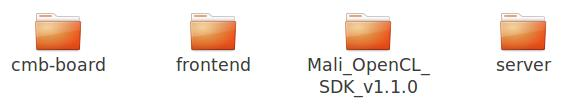
\includegraphics[width=0.8\textwidth, height=0.2\textwidth]{figs/workspace.jpg}
    \caption[Workspace folder structure]{Workspace folder structure}
    \label{fig:workspace}
\end{figure}

\begin{figure}
    \centering
    \begin{subfigure}[b]{0.2\textwidth}
        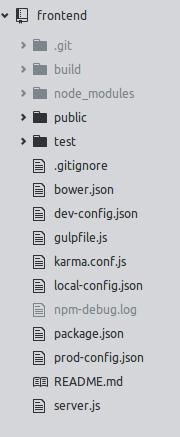
\includegraphics[width=\textwidth]{figs/frontend.jpg}
        \caption{Frontend}
        \label{fig:folders-frontend}
    \end{subfigure}
    ~ %add desired spacing between images, e. g. ~, \quad, \qquad, \hfill etc.
      %(or a blank line to force the subfigure onto a new line)
    \begin{subfigure}[b]{0.2\textwidth}
        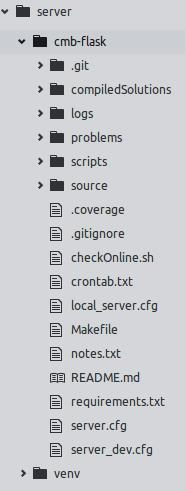
\includegraphics[width=\textwidth]{figs/server.jpg}
        \caption{Server}
        \label{fig:folders-server}
    \end{subfigure}
    ~ %add desired spacing between images, e. g. ~, \quad, \qquad, \hfill etc.
    %(or a blank line to force the subfigure onto a new line)
    \begin{subfigure}[b]{0.2\textwidth}
        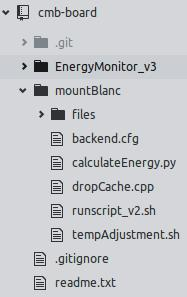
\includegraphics[width=\textwidth]{figs/backend.jpg}
        \caption{Backend}
        \label{fig:folders-backend}
    \end{subfigure}
    \caption{Folder structure}\label{fig:folder-structure}
\end{figure}

\clearpage

\begin{figure}
    \centering
    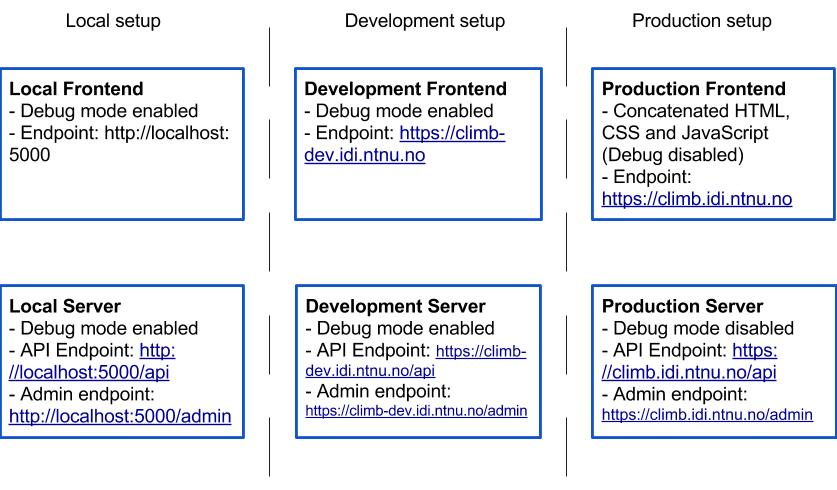
\includegraphics[width=0.9\textwidth, height=0.5\textwidth]{figs/setup-overview.jpg}
    \caption[General Overview of the Different Setup Options]{General Overview of the Different Setup Options}
    \label{fig:setup-overview}
\end{figure}

\section{Frontend Setup}
\label{sec:fsetup}
Figure \ref{fig:folders-frontend} shows the structure of the frontend code, and will be relevant in this section. Acquire the frontend code and create the folder structure shown in figure \ref{fig:folders-frontend} before starting setup. This section gathers the setup and handover information from the master thesis of Follan and Støa \cite{mt:T&S}, and is rewritten according to the proposed folder structure to make the setup easier.

\paragraph*{CMB Frontend Setup} \hfill \\
To build the frontend run the following command in the \textit{frontend/} directory:
\begin{lstlisting}[language=sh]
npm install
\end{lstlisting}
The command will install all the required packages with \textit{npm} \cite{m:npm}. The required packages is listed in a file called \textit{package.json}. After running the command, the required packages will be saved in a folder called \textit{node\_modules}. To build the system as it is used on the production server, the build tool \textit{gulp} \cite{m:gulp} is used with the following command in the \textit{frontend/} directory:
\begin{lstlisting}[language=sh]
gulp prod
\end{lstlisting}
The command will concatenate the HTML, CSS and JavaScript files which makes the code more efficient, and lowers the number of requests made when fetching data to the browser. However, since this concatenation reduces the number of source files, the code will be harder to debug. After running the commands, the frontend should be available at the URL \url{https://climb.idi.ntnu.no}, but keep in mind that it will not function properly before the server has been set up. The frontend will assume that a server API is available at \url{https://climb.idi.ntnu.no/api} to fetch data, which requires a running server as explained in section \ref{sec:ssetup}. To build the development version instead, stay in the \textit{frontend/} directory and run:
\begin{lstlisting}[language=sh]
gulp dev
\end{lstlisting}
The command will not concatenate the HTML, CSS and JavaScript files, which will make it easier to debug using developer tools in the browser. The frontend should now be available at \url{https://climb-dev.idi.ntnu.no}. The development frontend also requires a running server with an API available at \url{https://climb-dev.idi.ntnu.no/api}, as explained in section \ref{sec:ssetup}.

\paragraph*{Local Setup} \hfill \\
First, as above, run the following command in the \textit{frontend/} directory:
\begin{lstlisting}[language=sh]
npm install
\end{lstlisting}
The command will install all dependencies from listed in \textit{package.json}.
\noindent
To build the frontend for local development, run the following command in the \textit{frontend/} directory:
\begin{lstlisting}
gulp
\end{lstlisting}
The command will build the project as it is done on the development server, but the website is instead available at \url{http://localhost:5000}. This means that a local version of the server should also be run (described in section \ref{sec:ssetup}). The command will also watch for changes in the code, and for every change it will run the unit tests and rebuild the code. All gulp tasks are defined in the \textit{gulpfile.js}, and new tasks can be added there. New code or modifications to existing code should be done in the \textit{public/} folder

\paragraph*{Unit Tests and Linter} \hfill \\
To make the unit tests run correctly, all \textit{bower} \cite{m:bower} dependencies must be installed as mentioned in section \ref{sec:bs-cmb}. This is done by running the following command in the \textit{frontend/} directory:
\begin{lstlisting}[language=sh]
bower install
\end{lstlisting}
This will install all dependencies from the \textit{bower.json} file in the bower components folder. To run the tests, enter the \textit{frontend/} directory and run the tests through the \textit{gulp} task:
\begin{lstlisting}
gulp test
\end{lstlisting}
When the tests are run, a directory called \textit{coverage/} is automatically created within the \textit{frontend/} directory. This directory contains an HTML report of the test run.\\

To run the \textit{jshint} \cite{m:jshint} linter manually, run the following \textit{gulp task} in the \textit{frontend/} directory:
\begin{lstlisting}[language=sh]
gulp jshint
\end{lstlisting}
The command will report linter errors if any.

\section{Server Setup}
\label{sec:ssetup}
The directory structure for the server can be seen in figure \ref{fig:folders-server}. Acquire the server code and create the folder structure in figure \ref{fig:folders-server} before starting setup. The paragraphs "Installation and Configuration", "Database Setup and Migration" and "Unit Tests and Linter" are setup information created by Follan and Støa. The paragraphs are rewritten and complemented using the proposed folder structure to make the setup process easier.

\paragraph*{Virtual Environment and Dependencies} \hfill \\
A Python Virtual Environment (VE) \cite{m:virtualenv} should be installed and used when developing and running the server code. When installed, create a new VE by running the following command in the \textit{server/} directory:
\begin{lstlisting}[language=sh]
virtualenv venv
\end{lstlisting}
The command will create the folder structure \textit{venv} within the \textit{server/} directory. One need to activate the VE to install packages and use the packages installed within it. The Unix command \textit{source} is used to activate the VE. An example from the \textit{server/} directory is:
\begin{lstlisting}[language=sh]
source ./venv/bin/activate
\end{lstlisting}

To install all required packages needed on the server, activate the VE and use \textit{pip} \cite{m:pip} to install the required packages within the VE. All required packages is listed in the \textit{requirements.txt} file, and is installed by running the following command from the \textit{server/cmb-server/} directory:
\begin{lstlisting}[language=sh]
pip install -r requirements.txt
\end{lstlisting}
The above command will install all required Python dependencies needed for correct execution of the server. Installation of requirements needs to be done both when developing locally and when setting up a new CMB server. \\

To deactivate the VE, execute the following command anywhere:
\begin{lstlisting}[language=sh]
deactivate
\end{lstlisting}

\paragraph*{Installation and Configuration} \hfill \\
To correctly compile the uploaded solutions on the server, a \textit{Mali OpenCL SDK} \cite{m:mali} library is needed. It is recommended to install it as shown in figure \ref{fig:workspace}. It is also a requirement to create a directory called \textit{workspace/} within the extracted folder of the Mali OpenCL SDK. The CMB server also needs OpenMP 4.0, gcc-4.9 and g++-4.9 to compile the uploaded programs correctly. The following steps installs the required compilers and libraries:
\begin{lstlisting}
sudo apt-get-repository ppa:ubuntu-toolchain-r/test
sudo apt-get update
sudo apt-get install gcc-4.9 g++-4.9
sudo apt-get install build-essential
\end{lstlisting}

Uncomplicated Firewall (UFW) \cite{m:ufw} and Fail2Ban \cite{m:f2b} are installed and configured by running the commands below:
\begin{lstlisting}
sudo apt-get install fail2ban
sudo ufw allow 80
sudo ufw allow 443
sudo ufw enable
\end{lstlisting}
UFW should already be present, and does not need installation. The second and third command above allows requests to port 80 and 443. That is, all HTTP and HTTPS request should be allowed to pass to the server. Fail2Ban should work out of the box.\\

Some environment variables need to be setup to configure a CMB server correctly. Firstly, the Unix environment variable \textit{APPLICATIONS\_SETTINGS} need to be set. This environment variable points to a file that contains application specific variables, depending on if the server is either a production, development or a local server. The files \textit{server.cfg}, \textit{server\_dev.cfg} and \textit{local\_server.cfg} present in the directory \textit{server/cmb-flask/} represents the application settings for a production, development or a local server respectively. For example, the IP address of a backend board, the path for the Mali OpenCL SDK, the database URI and the server port is all present in the configuration files among other variables. Appendix \ref{appendix/config} gives an example of how the file \textit{local\_server.cfg} might look like. It is very important to enter these values correctly. \\

The next environment variables that need to be set is \textit{CMB\_MAIL\_USERNAME}, \textit{CMB\_MAIL\_PASSWORD}, \textit{CMB\_SECRET\_KEY} and \textit{CMB\_TOKEN\_SECRET}. The variables \textit{CMB\_MAIL\_USERNAME} and \textit{CMB\_MAIL\_PASSWORD} are used to send an email to the CMB administrators when an error occurs, which is crucial if setting up a production environment. The variables \textit{CMB\_SECRET\_KEY} and \textit{CMB\_TOKEN\_SECRET} is used for session token generation, authenticating messages and more.  When developing locally, these variables can stay unchanged and can be copied from the file \textit{local\_server.sh} present in the directory \textit{cmb-flask/scripts/}. If setting up a development or production server, contact the CMB team, and they will provide the information to set these variables correctly. It is recommended to enter the variables into \textit{\$HOME/bash\_profile} or some similar file that loads the environment variables when starting up a new shell. Run the following command from the directory \textit{server/cmb-flask/scripts/} to start either a development or production server:
\begin{lstlisting}
./init_cmb start
\end{lstlisting}
The command will start the whole CMB system, including the frontend and \textit{push.py}. Keep in mind that the system will not function correctly before a backend has been setup, as described in section \ref{sec:bsetup}. The above command also allows the arguments \textit{stop} and \textit{restart} as well, to stop or restart the CMB system respectively. The above command is the recommended way of starting either a production or development server. To start a local server, run the following command in the \textit{server/cmb-flask/source/} directory:
\begin{lstlisting}
python server.py start
\end{lstlisting}
This will start the server without \textit{Gunicorn} \cite{m:guni}. Running the server without Gunicorn makes it easier to debug, as only a single instance of the server is running. However, it is possible to launch the CMB locally with the \textit{init\_cmb} script locally as well if wanted. No matter the method of running the server, it will create a callable API at endpoint \url{https://localhost:5000}. It is important to initialize the database (see below) before running the server the first time.

\paragraph*{Database Setup and Migration} \hfill \\
To clear and initialize a database for a new server, run the following command in the directory \textit{server/cmb-flask/}:
\begin{lstlisting}
python init_db.py
\end{lstlisting}
If there is a modification to the database models (read table schema), one need to \textit{migrate} \footnote{Migration is the task of updating or reverting a database schema while trying to preserve the data that might be present in the database.} the database. Migration happens by creating a migration script, generated by running the following command in from the \textit{server/cmb-flask/source/} directory:
\begin{lstlisting}
python server.py db migrate -m "some message."
\end{lstlisting}
This will create a new directory within \textit{server/cmb-flask/source/} called \textit{migrations} if not present, with the auto generated migrations script within. To launch the migration script and alter the database table schema, stay in the directory \textit{server/cmb-flask/source/} and run:
\begin{lstlisting}
python server.py db upgrade
\end{lstlisting}
On the production and development servers, this is done automatically through Jenkins when there is a change to the database tables. The migration script is also added to the git repository so that the above step can be executed manually. \\


\paragraph*{Unit Tests and Linter} \hfill \\
After installing and activating the virtual environment above, make sure all required packages from \textit{requirements.txt} is installed. From the directory \textit{server/cmb-flask/source/}, run the following command:
\begin{lstlisting}
nosetests --with-coverage --cover-package=admin,routes,cmb_utils,server,database tests/*.py
\end{lstlisting}
This will run automatic unit tests with \textit{nose} \cite{m:nose} for all tests present in the directory \textit{server/cmb-flask/source}. It will also generate a cover report, with an extensive overview of the code covered by the tests. If developing a new test, it might be useful running just a single test. To run a single test, execute the following command the \textit{server/cmb-flask/source/} folder:
\begin{lstlisting}
nosetest tests/problems_test.py
\end{lstlisting}
This will run the tests present in the \textit{problems\_test.py} file. One can simply run another test set by changing the file name to another file present in the \textit{server/cmb-flask/source/tests/} directory. \\
\noindent
To run the \textit{flake8} linter, stay in the \textit{server/cmb-flask/source/} directory and run:
\begin{lstlisting}
flake8 .
\end{lstlisting}
The terminal window will report potential errors.

\section{Backend Setup}
\label{sec:bsetup}
This section explains the setup of a new Odroid-XU3 board with the folder structure equal to the one in figure \ref{fig:folders-backend}. The folder structure is relevant when setting up the CMB board code as explained below. The paragraph "CMB Setup" contains instructions and information made by Follan and Støa, which is further complemented (uninstalling \textit{lightdm} \cite{m:lightdm}) and rewritten to make setup easier.

\paragraph*{Odroid-XU3 Setup} \hfill \\
A new Odroid-XU3 board should have a fresh installation of Xubuntu installed available at the Odroid website \cite{m:odroid}. The Xubuntu installation information given here is inspired by the information stated at the Odroid website \cite{m:odroid-i}. The Odroid-XU3 can either boot from a MicroSD card or a special module called eMMC module. The eMMC module needs to be connected to a eMMC module reader as seen in the figure \ref{fig:emmc} to be able to flash. A Unix operating system is assumed used when flashing the OS image onto an eMMC module or a MicroSD. For flashing of OS images onto MicroSD like media using Windows, refer to the Odroid website \cite{m:odroid}. After downloading a new Operating System image, flash the connected MicroSD card or eMMC module with the following commands within the folder where the image is downloaded:
\begin{lstlisting}
unxz some-xubuntu-image-file.img.xz
sudo dd if=/dev/zero of=</dev/path/of/card> bs=4M conv=fsync
sudo dd if=<some-xubuntu-image-file.img> of=</dev/path/of/card> bs=4M conv=fsync
sync
\end{lstlisting}
The path of the MicroSD card or eMMC module can be found by monitoring the directory \textit{/dev/} before and after connecting the device. The connected device will appear as sdX, where X is some alphabetical character. As mentioned, CMB uses the EnergyMonitor program to measure energy consumption, and it is important to check that the downloaded OS image supports the EnergyMonitor program.\\

\begin{figure}
    \centering
    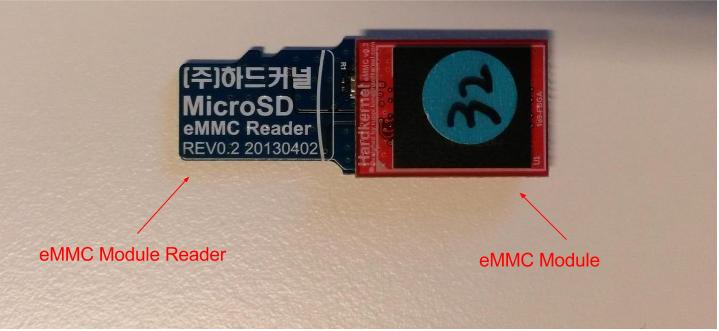
\includegraphics[width=0.9\textwidth, height=0.4\textwidth]{figs/emmc.jpg}
    \caption[eMMC Module Reader and the eMMC Module]{eMMC Module Reader and the eMMC Module}
    \label{fig:emmc}
\end{figure}

\noindent
After installing the OS, connect either the MicroSD or eMMC module to the board\footnote{Check out \url{http://odroid.com/dokuwiki/doku.php?id=en:xu3_bootmode_configuration} on how to toggle between booting from eMMC module and MicroSD.}. Then boot and connect the Odroid-XU3 to a monitor either trough mini-HDMI or a DisplayPort. An automatic login will happen to a user called \textit{odroid}. Open a terminal window and create two more users by running the following commands:
\begin{lstlisting}
useradd climber
passwd climber
useradd worker
\end{lstlisting}
This creates two users, \textit{climber} and \textit{worker}. When prompted for a password for the \textit{climber} user, enter the password given to you by the CMB team. These two users are needed to execute commands and run programs through the server. Additionally, enter the following line to the end of the file \textit{sudoers} located in the directory \textit{/etc/}:
\begin{lstlisting}
...
climber    ALL=(worker) NOPASSWD: ALL
...
\end{lstlisting}
The line will make sure that the \textit{worker} user have the privileges to execute the uploaded programs. The command \textit{visodu} should be used to add the line to the \textit{sudoers} file. \\

The backend should install OpenSSH and OpenSSH Server if not already installed \cite{m:openssh}. The two services can be installed and configured to CMB by executing the following commands:
\begin{lstlisting}
sudo apt-get install ssh-client
sudo apt-get install ssh-server
ssh-keygen -t rsa
ssh-copy-id username@ip-to-server
\end{lstlisting}
When prompted for something, just hit enter. After executing the commands above, login to the board can happen without entering a password. This will make sure that the server does not get prompted for a password when it needs to execute scripts at the backend. You should not be prompted for a password when logging into the board from the server after executing these commands. \\

Uncomplicated Firewall (UFW) and Fail2Ban are installed much the same way as on the server. Execute the following commands to install and configure both services:
\begin{lstlisting}
sudo apt-get install fail2ban
sudo ufw allow from 127.241.0.0/16
sudo ufw enable
\end{lstlisting}
The board should not be accessible from outside the NTNU network, which this UFW configuration ensures.

\paragraph*{CMB Setup} \hfill \\
Follan and Støa reported the CMB backend setup in their Master thesis \cite{mt:T&S}. The commands to setup the CMB backend code is repeated here, and extended with the removal of \textit{lightdm} \cite{m:lightdm}. Log in as \textit{climber} at the board through SSH and fetch the backend code from Bitbucket (clone the repository with git), and run the following commands to correctly setup the CMB backend: \\

\begin{lstlisting}
# Link binary
sudo ln -sf /lib/ld-linux-armhf.so.3 /lib/ld-linux.so.3
# programs and packages used by runscript_v2.sh, EnergyMonitor and
calculateEnergy.py.
sudo apt-get install python-scipy time qt4-default libqwt-dev
# install g++ and gcc 4.9 to support OpenMP 4.0
sudo add-apt-repository ppa:ubuntu-toolchain-r/test
sudo apt-get update
sudo apt-get install gcc-4.9 g++-4.9
sudo apt-get install build-essential
# add following line to /etc/rc.local. This script is run automatically on boot,
# and is needed for tempAdjustment to read current temperature.
# Permissions are reset when rebooting.
chmod +r /sys/devices/10060000.tmu/temp
# These are needed by the EnergyMonitor_v3.
# Make sure executable name is "EnergyMonitor"
cd cmb-board/EnergyMonitor_v3
qmake
make
# Remove lightdm for accurate energy readings
sudo apt-get purge lightdm
# compile dropCache.cpp to dropCache and make it an auxiliary executable.
# dropCache is responsible for clearing the cache before running a program.
cd ~/cmb-board/mountBlanc
g++ -O2 dropCache.cpp -o dropCache
chmod 4710 dropCache
\end{lstlisting}
Download the Mali OpenCL SDK v1.1 and copy the folders \textit{common}, \textit{lib} and \textit{include} into the directory \textit{cmb-board}. The folders can also be transferred from the server.

\end{appendices}

\end{document}
